\documentclass[twoside]{article}
%DIF LATEXDIFF DIFFERENCE FILE



%DIF 3c3
%DIF < \usepackage{aistats2022}
%DIF -------
%\usepackage{aistats2022} %DIF > 
%DIF -------
% If your paper is accepted, change the options for the package
% aistats2022 as follows:
%
%DIF 7c7
%DIF < %\usepackage[accepted]{aistats2022}
%DIF -------
\usepackage[accepted]{aistats2022} %DIF > 
%DIF -------
%
% This option will print headings for the title of your paper and
% headings for the authors names, plus a copyright note at the end of
% the first column of the first page.

% If you set papersize explicitly, activate the following three lines:
%DIF 14-17c14-16
%DIF < %\special{papersize = 8.5in, 11in}
%DIF < %\setlength{\pdfpageheight}{11in}
%DIF < %\setlength{\pdfpagewidth}{8.5in}
%DIF < 
%DIF -------
\special{papersize = 8.5in, 11in} %DIF > 
\setlength{\pdfpageheight}{11in} %DIF > 
\setlength{\pdfpagewidth}{8.5in} %DIF > 
%DIF -------
% If you use natbib package, activate the following three lines:
%DIF 19-21c18-20
%DIF < %\usepackage[round]{natbib}
%DIF < %\renewcommand{\bibname}{References}
%DIF < %\renewcommand{\bibsection}{\subsubsection*{\bibname}}
%DIF -------
\usepackage[round,authoryear]{natbib} %DIF > 
\renewcommand{\bibname}{References} %DIF > 
\renewcommand{\bibsection}{\subsubsection*{\bibname}} %DIF > 
%DIF -------

% If you use BibTeX in apalike style, activate the following line:
%\bibliographystyle{apalike}

%DIF 26a25-30
% page number margin %DIF > 
 %DIF > 
%\setlength{\footskip}{10pt} %DIF > 
 %DIF > 
\usepackage[hidelinks]{hyperref} %DIF > 
 %DIF > 
%DIF -------
\usepackage{algpseudocode}
\usepackage{amsmath}
\usepackage{graphicx}
\usepackage{enumerate}
%DIF 30d35
%DIF < \usepackage[square,numbers]{natbib}
%DIF -------
\usepackage{url}
\usepackage{enumitem}

%DIF 34-38d38
%DIF < \newcommand\Algphase[1]{%
%DIF < \vspace*{-.7\baselineskip}\Statex\hspace*{\dimexpr-\algorithmicindent-2pt\relax}\rule{\textwidth}{0.4pt}%
%DIF < \Statex\hspace*{-\algorithmicindent}\textbf{#1}%
%DIF < \vspace*{-.7\baselineskip}\Statex\hspace*{\dimexpr-\algorithmicindent-2pt\relax}\rule{\textwidth}{0.4pt}%
%DIF < }
%DIF -------

%DIF 40a39
 %DIF > 
%DIF -------
\usepackage{amsmath,amssymb,amsthm,bm,mathtools}
\usepackage{algorithm}
\usepackage{dsfont,multirow,hyperref,setspace,enumerate}
%DIF 43c43
%DIF < \hypersetup{colorlinks,linkcolor={blue},citecolor={blue},urlcolor={black}}
%DIF -------
\hypersetup{colorlinks,linkcolor=blue,citecolor=blue,urlcolor={black}} %DIF > 
%DIF -------
\usepackage{lscape}
\usepackage{afterpage}
\usepackage{hyperref}

%DIF 48a48-62
\usepackage{microtype} %DIF > 
\usepackage{wrapfig} %DIF > 
\allowdisplaybreaks %DIF > 
\usepackage{algorithm} %DIF > 
\usepackage{algpseudocode} %DIF > 
 %DIF > 
\usepackage{textcomp} %DIF > 
\usepackage{stfloats} %DIF > 
\usepackage{verbatim} %DIF > 
\usepackage{array} %DIF > 
 %DIF > 
\usepackage{tabularx,booktabs} %DIF > 
\newcolumntype{Y}{>{\centering\arraybackslash}X} %DIF > 
 %DIF > 
 %DIF > 
%DIF -------
\theoremstyle{definition}
\newtheorem{thm}{Theorem}
\newtheorem{lem}{Lemma}
\newtheorem{prop}{Proposition}[section]
\newtheorem{pro}{Property}
%DIF 53c68
%DIF < \newtheorem{cor}{Corollary}[section]
%DIF -------
\newtheorem{cor}{Corollary} %DIF > 
%DIF -------

\theoremstyle{definition}
\newtheorem{assumption}{Assumption}
\newtheorem{defn}{Definition}
\newtheorem{example}{Example}
\newtheorem{rmk}{Remark}
\newtheorem{condition}{Condition}
\newtheorem{conjecture}{Conjecture}
\newtheorem{property}{Property}
%DIF 63a78
\newtheorem{hypothesis}{Hypothesis} %DIF > 
%DIF -------

\newtheorem{innercustomgeneric}{\customgenericname}
\providecommand{\customgenericname}{}
\newcommand{\newcustomtheorem}[2]{%
  \newenvironment{#1}[1]
  {%
   \renewcommand\customgenericname{#2}%
   \renewcommand\theinnercustomgeneric{##1}%
   \innercustomgeneric
  }
  {\endinnercustomgeneric}
}

%DIF 76a92
 %DIF > 
%DIF -------
\newcustomtheorem{customexample}{Example}

\usepackage{appendix}
%DIF 79a96-97
\usepackage{fullpage}  %DIF > 
\usepackage{microtype} %DIF > 
%DIF -------
\usepackage{wrapfig}
\mathtoolsset{showonlyrefs}

\newcommand{\of}[1]{\left(#1\right)}
\newcommand{\off}[1]{\left[#1\right]}
\newcommand{\offf}[1]{\left\{#1\right\}}
\newcommand{\aabs}[1]{\left|#1\right|}
\newcommand{\ang}[1]{\left\langle#1\right\rangle}

%DIF 88a107-108
\newcommand{\distgap}{D_{\ell_2}} %DIF > 
\newcommand{\Mat}{\text{Mat}} %DIF > 
%DIF -------

%DIF 89-93d110
%DIF < \usepackage{algpseudocode,algorithm}
%DIF < \algnewcommand\algorithmicinput{\textbf{Input:}}
%DIF < \algnewcommand\algorithmicoutput{\textbf{Output:}}
%DIF < \algnewcommand\INPUT{\item[\algorithmicinput]}
%DIF < \algnewcommand\OUTPUT{\item[\algorithmicoutput]}
%DIF -------

\def\ci{\perp\!\!\!\perp}

%DIF 97c113
%DIF < \def\fixme#1#2{\textbf{\color{red}[FIXME (#1): #2]}}
%DIF -------
 %DIF > 
%DIF -------
\usepackage{booktabs}
\newcommand\doubleRule{\toprule\toprule}
\allowdisplaybreaks

\newcommand*{\KeepStyleUnderBrace}[1]{%f
  \mathop{%
    \mathchoice
    {\underbrace{\displaystyle#1}}%
    {\underbrace{\textstyle#1}}%
    {\underbrace{\scriptstyle#1}}%
    {\underbrace{\scriptscriptstyle#1}}%
  }\limits
}
%DIF 111d127
%DIF < \newcommand{\anglegap}{\text{Angle}}
%DIF -------


%DIF 114-115d129
%DIF < \usepackage{xr}
%DIF < % this is for overleaf cross reference
%DIF -------

%DIF 117-123d130
%DIF < \newcommand*{\myexternaldocument}[1]{%
%DIF <     \externaldocument{#1}%
%DIF <     \addFileDependency{#1.tex}%
%DIF <     \addFileDependency{#1.aux}%
%DIF < }
%DIF < %\myexternaldocument{supplement}
%DIF < 
%DIF -------
\input macros.tex
%DIF 125a131
 %DIF > 
%DIF -------
\newcommand*{\Scale}[2][4]{\scalebox{#1}{$#2$}}%
\setlength\parindent{0pt} %DIF > 
\usepackage[parfill]{parskip} %DIF > 
\usepackage{algorithm} %DIF > 
\usepackage{algpseudocode} %DIF > 
\usepackage{amsmath} %DIF > 
 %DIF > 
 %DIF > 
\DeclarePairedDelimiter{\ceil}{\lceil}{\rceil} %DIF > 
\DeclarePairedDelimiter{\floor}{\lfloor}{\rfloor} %DIF > 
 %DIF > 
\algnewcommand\algorithmicinput{\textbf{Input:}} %DIF > 
\algnewcommand\algorithmicoutput{\textbf{Output:}} %DIF > 
\algnewcommand\INPUT{\item[\algorithmicinput]} %DIF > 
\algnewcommand\OUTPUT{\item[\algorithmicoutput]} %DIF > 
 %DIF > 
\newcommand\Algphase[1]{% %DIF > 
\vspace*{-.7\baselineskip}\Statex\hspace*{\dimexpr-\algorithmicindent-2pt\relax}\rule{\textwidth}{0.4pt}% %DIF > 
\Statex\hspace*{-\algorithmicindent}\textbf{#1}% %DIF > 
\vspace*{-.7\baselineskip}\Statex\hspace*{\dimexpr-\algorithmicindent-2pt\relax}\rule{\textwidth}{0.4pt}% %DIF > 
} %DIF > 
\usepackage{caption} %DIF > 
\def\fixme#1#2{\textbf{\color{red}[FIXME (#1): #2]}} %DIF > 
%DIF PREAMBLE EXTENSION ADDED BY LATEXDIFF
%DIF UNDERLINE PREAMBLE %DIF PREAMBLE
\RequirePackage[normalem]{ulem} %DIF PREAMBLE
\RequirePackage{color}\definecolor{RED}{rgb}{1,0,0}\definecolor{BLUE}{rgb}{0,0,1} %DIF PREAMBLE
\providecommand{\DIFaddtex}[1]{{\protect\color{blue}\uwave{#1}}} %DIF PREAMBLE
\providecommand{\DIFdeltex}[1]{{\protect\color{red}\sout{#1}}}                      %DIF PREAMBLE
%DIF SAFE PREAMBLE %DIF PREAMBLE
\providecommand{\DIFaddbegin}{} %DIF PREAMBLE
\providecommand{\DIFaddend}{} %DIF PREAMBLE
\providecommand{\DIFdelbegin}{} %DIF PREAMBLE
\providecommand{\DIFdelend}{} %DIF PREAMBLE
%DIF FLOATSAFE PREAMBLE %DIF PREAMBLE
\providecommand{\DIFaddFL}[1]{\DIFadd{#1}} %DIF PREAMBLE
\providecommand{\DIFdelFL}[1]{\DIFdel{#1}} %DIF PREAMBLE
\providecommand{\DIFaddbeginFL}{} %DIF PREAMBLE
\providecommand{\DIFaddendFL}{} %DIF PREAMBLE
\providecommand{\DIFdelbeginFL}{} %DIF PREAMBLE
\providecommand{\DIFdelendFL}{} %DIF PREAMBLE
%DIF HYPERREF PREAMBLE %DIF PREAMBLE
\providecommand{\DIFadd}[1]{\texorpdfstring{\DIFaddtex{#1}}{#1}} %DIF PREAMBLE
\providecommand{\DIFdel}[1]{\texorpdfstring{\DIFdeltex{#1}}{}} %DIF PREAMBLE
\newcommand{\DIFscaledelfig}{0.5}
%DIF HIGHLIGHTGRAPHICS PREAMBLE %DIF PREAMBLE
\RequirePackage{settobox} %DIF PREAMBLE
\RequirePackage{letltxmacro} %DIF PREAMBLE
\newsavebox{\DIFdelgraphicsbox} %DIF PREAMBLE
\newlength{\DIFdelgraphicswidth} %DIF PREAMBLE
\newlength{\DIFdelgraphicsheight} %DIF PREAMBLE
% store original definition of \includegraphics %DIF PREAMBLE
\LetLtxMacro{\DIFOincludegraphics}{\includegraphics} %DIF PREAMBLE
\newcommand{\DIFaddincludegraphics}[2][]{{\color{blue}\fbox{\DIFOincludegraphics[#1]{#2}}}} %DIF PREAMBLE
\newcommand{\DIFdelincludegraphics}[2][]{% %DIF PREAMBLE
\sbox{\DIFdelgraphicsbox}{\DIFOincludegraphics[#1]{#2}}% %DIF PREAMBLE
\settoboxwidth{\DIFdelgraphicswidth}{\DIFdelgraphicsbox} %DIF PREAMBLE
\settoboxtotalheight{\DIFdelgraphicsheight}{\DIFdelgraphicsbox} %DIF PREAMBLE
\scalebox{\DIFscaledelfig}{% %DIF PREAMBLE
\parbox[b]{\DIFdelgraphicswidth}{\usebox{\DIFdelgraphicsbox}\\[-\baselineskip] \rule{\DIFdelgraphicswidth}{0em}}\llap{\resizebox{\DIFdelgraphicswidth}{\DIFdelgraphicsheight}{% %DIF PREAMBLE
\setlength{\unitlength}{\DIFdelgraphicswidth}% %DIF PREAMBLE
\begin{picture}(1,1)% %DIF PREAMBLE
\thicklines\linethickness{2pt} %DIF PREAMBLE
{\color[rgb]{1,0,0}\put(0,0){\framebox(1,1){}}}% %DIF PREAMBLE
{\color[rgb]{1,0,0}\put(0,0){\line( 1,1){1}}}% %DIF PREAMBLE
{\color[rgb]{1,0,0}\put(0,1){\line(1,-1){1}}}% %DIF PREAMBLE
\end{picture}% %DIF PREAMBLE
}\hspace*{3pt}}} %DIF PREAMBLE
} %DIF PREAMBLE
\LetLtxMacro{\DIFOaddbegin}{\DIFaddbegin} %DIF PREAMBLE
\LetLtxMacro{\DIFOaddend}{\DIFaddend} %DIF PREAMBLE
\LetLtxMacro{\DIFOdelbegin}{\DIFdelbegin} %DIF PREAMBLE
\LetLtxMacro{\DIFOdelend}{\DIFdelend} %DIF PREAMBLE
\DeclareRobustCommand{\DIFaddbegin}{\DIFOaddbegin \let\includegraphics\DIFaddincludegraphics} %DIF PREAMBLE
\DeclareRobustCommand{\DIFaddend}{\DIFOaddend \let\includegraphics\DIFOincludegraphics} %DIF PREAMBLE
\DeclareRobustCommand{\DIFdelbegin}{\DIFOdelbegin \let\includegraphics\DIFdelincludegraphics} %DIF PREAMBLE
\DeclareRobustCommand{\DIFdelend}{\DIFOaddend \let\includegraphics\DIFOincludegraphics} %DIF PREAMBLE
\LetLtxMacro{\DIFOaddbeginFL}{\DIFaddbeginFL} %DIF PREAMBLE
\LetLtxMacro{\DIFOaddendFL}{\DIFaddendFL} %DIF PREAMBLE
\LetLtxMacro{\DIFOdelbeginFL}{\DIFdelbeginFL} %DIF PREAMBLE
\LetLtxMacro{\DIFOdelendFL}{\DIFdelendFL} %DIF PREAMBLE
\DeclareRobustCommand{\DIFaddbeginFL}{\DIFOaddbeginFL \let\includegraphics\DIFaddincludegraphics} %DIF PREAMBLE
\DeclareRobustCommand{\DIFaddendFL}{\DIFOaddendFL \let\includegraphics\DIFOincludegraphics} %DIF PREAMBLE
\DeclareRobustCommand{\DIFdelbeginFL}{\DIFOdelbeginFL \let\includegraphics\DIFdelincludegraphics} %DIF PREAMBLE
\DeclareRobustCommand{\DIFdelendFL}{\DIFOaddendFL \let\includegraphics\DIFOincludegraphics} %DIF PREAMBLE
%DIF END PREAMBLE EXTENSION ADDED BY LATEXDIFF

\begin{document}

% If your paper is accepted and the title of your paper is very long,
% the style will print as headings an error message. Use the following
% command to supply a shorter title of your paper so that it can be
% used as headings.
%
%\runningtitle{I use this title instead because the last one was very long}

% If your paper is accepted and the number of authors is large, the
% style will print as headings an error message. Use the following
% command to supply a shorter version of the authors names so that
% they can be used as headings (for example, use only the surnames)
%
%\runningauthor{Surname 1, Surname 2, Surname 3, ...., Surname n}

\DIFdelbegin %DIFDELCMD < \twocolumn[
%DIFDELCMD < 

%DIFDELCMD < \aistatstitle{Multiway Spherical Clustering via Degree-Corrected\\ Tensor Block Models}
%DIFDELCMD < 

%DIFDELCMD < \aistatsauthor{ Author 1 \And Author 2 \And  Author 3 }
%DIFDELCMD < 

%DIFDELCMD < \aistatsaddress{ Institution 1 \And  Institution 2 \And Institution 3 } ]
%DIFDELCMD < %%%
\DIFdelend \DIFaddbegin \twocolumn[

\aistatstitle{Multiway Spherical Clustering via Degree-Corrected\\ Tensor Block Models}

\aistatsauthor{ Jiaxin Hu \And Miaoyan Wang }

\aistatsaddress{ University of Wisconsin -- Madison \And  University of Wisconsin -- Madison} ]
\DIFaddend 

\begin{abstract}
We consider the problem of multiway clustering in the presence of unknown degree heterogeneity. Such data problems arise commonly in applications such as recommendation system, neuroimaging, community detection, and hypergraph partitions in social networks. The allowance of degree heterogeneity provides great flexibility in clustering models, but the extra complexity poses significant challenges in both statistics and computation. Here, we develop a degree-corrected tensor block model with estimation accuracy guarantees. We present the phase transition of clustering performance based on the notion of angle separability, and we characterize three signal-to-noise regimes corresponding to different statistical-computational behaviors. In particular, we demonstrate that an intrinsic statistical-to-computational gap emerges only for tensors of order three or greater. Further, we develop an efficient polynomial-time algorithm that provably achieves exact clustering under mild signal conditions. The efficacy of our procedure is demonstrated through both simulations and analyses of Peru Legislation dataset.  
\DIFdelbegin %DIFDELCMD < 

%DIFDELCMD < %%%
\DIFdelend \end{abstract}


\section{\DIFdelbegin \DIFdel{Introduction}\DIFdelend \DIFaddbegin \DIFadd{INTRODUCTION}\DIFaddend }\label{sec:intro}
\DIFdelbegin %DIFDELCMD < 

%DIFDELCMD < %%%
%DIF < {\color{blue} \textbor{Below are my thoughts(main points I want to involve) about the introduction structure. I will elaborate each statement. }}
%DIFDELCMD < 

%DIFDELCMD < %%%
\DIFdelend Multiway arrays have been widely collected in various fields including social networks \citep{anandkumar2014tensor}, neuroscience \citep{wang2017bayesian}, and computer science \citep{koniusz2016sparse}. Tensors effectively represent the multiway data and serve as the foundation in higher-order data analysis. One data example is from multi-tissue multi-individual gene expression study~\citep{wang2019three,hore2016tensor}, where the data tensor consists of expression measurements indexed by (gene, individual, tissue) triplets. Another example is \emph{hypergraph} network~\DIFdelbegin \DIFdel{\mbox{%DIFAUXCMD
\cite{ghoshdastidar2017uniform,ghoshdastidar2017consistency,ahn2019community,ke2019community} }\hspace{0pt}%DIFAUXCMD
}\DIFdelend \DIFaddbegin \DIFadd{\mbox{%DIFAUXCMD
\citep{ghoshdastidar2017uniform,ghoshdastidar2017consistency,ahn2019community,ke2019community} }\hspace{0pt}%DIFAUXCMD
}\DIFaddend in social science. A $K$-uniform hypergraph can be naturally represented as an order-$K$ tensor, where each entry indicates the presence of $K$-way hyperedge among nodes (a.k.a.\ entities). In both examples, identifying the similarity among tensor entities is important for scientific discovery. 


%DIF < To overcome the high-dimensionality, low-rankness is one of the popular structures utilized in tensor data analysis. Specifically, for an order-$K$ tensor $
%DIF < \tY$ with low-rank, we have the following decomposition:
%DIF < \begin{equation}\label{eq:low_rank}
 %DIF <    \tY = \tS \times_1 \mM_1 \cdots \times_K \mM_K, 
%DIF < \end{equation}
%DIF < where $\tS$ is the low-dimensional core tensor, $\mM_1, ..., \mM_K$ refer to the factor matrices, and $\times_k$ denotes the tensor-to-matrix product. 
\DIFdelbegin %DIFDELCMD < 

%DIFDELCMD < %%%
\DIFdel{This paper studies }\DIFdelend \DIFaddbegin \DIFadd{We study }\DIFaddend the problem of multiway clustering based on a data tensor. The goal of multiway clustering is to identify a checkerboard structure from a noisy data tensor. \DIFdelbegin \DIFdel{Fig.}\DIFdelend \DIFaddbegin \DIFadd{Figure}\DIFaddend ~\ref{fig:intro} illustrates the noisy tensor and the underlying \DIFaddbegin \DIFadd{checkerboard }\DIFaddend structures discovered by multiway clustering methods. \DIFdelbegin \DIFdel{The checkerboard structure serves as a meta tool to many popular structures including the low-rankness~\mbox{%DIFAUXCMD
\citep{young2018universality}}\hspace{0pt}%DIFAUXCMD
, latent space models~\mbox{%DIFAUXCMD
\citep{wang2018learning}}\hspace{0pt}%DIFAUXCMD
, and isotonic models~\mbox{%DIFAUXCMD
\citep{pananjady2020isotonic}}\hspace{0pt}%DIFAUXCMD
. }\DIFdelend In the hypergraph example, the multiway clustering aims to identify the underlying block partition of nodes based on their higher-order connectivities; therefore, we also refer to the clustering as \emph{higher-order clustering}. The most common model for higher-order clustering is called \emph{tensor block model} (TBM)~\DIFdelbegin \DIFdel{\mbox{%DIFAUXCMD
\cite{chi2020provable,wang2019multiway}}\hspace{0pt}%DIFAUXCMD
}\DIFdelend \DIFaddbegin \DIFadd{\mbox{%DIFAUXCMD
\citep{wang2019multiway}}\hspace{0pt}%DIFAUXCMD
}\DIFaddend , which extends the usual matrix stochastic block model~\citep{abbe2017community} to tensors. %DIF < The analysis tools developed for matrices,
\DIFdelbegin \DIFdel{The matrix }\DIFdelend \DIFaddbegin \DIFadd{Matrix }\DIFaddend analysis tools, however, are sub-optimal for higher-order clustering. Developing tensor tools for solving block models has received increased interest recently~\DIFdelbegin \DIFdel{\mbox{%DIFAUXCMD
\citep{han2020exact, wang2019multiway}}\hspace{0pt}%DIFAUXCMD
}\DIFdelend \DIFaddbegin \DIFadd{\mbox{%DIFAUXCMD
\citep{ wang2019multiway,chi2020provable,han2020exact}}\hspace{0pt}%DIFAUXCMD
}\DIFaddend . 


\DIFdelbegin \DIFdel{TBM }\DIFdelend \DIFaddbegin \DIFadd{Classical tensor block model }\DIFaddend suffers from drawbacks to model real world data in spite of the popularity. The key underlying assumption of block model is that all nodes in the same community are exchangeable; i.e., the nodes have no \DIFdelbegin \DIFdel{individual effects }\DIFdelend \DIFaddbegin \DIFadd{individual-specific parameters }\DIFaddend apart from the \DIFdelbegin \DIFdel{block effects}\DIFdelend \DIFaddbegin \DIFadd{community-specific parameters}\DIFaddend . However, the exchangeability assumption is often non-realistic. Each node may contribute to the data variation by its own multiplicative effect. \DIFaddbegin \DIFadd{We call the unequal node-specific effects the }\emph{\DIFadd{degree heterogeneity}}\DIFadd{. }\DIFaddend Such degree heterogeneity appears commonly in social networks. \DIFaddbegin \DIFadd{Ignoring the degree heterogeneity may seriously mislead the clustering results. }\DIFaddend For example, regular block model fails to model the \DIFaddbegin \DIFadd{member affiliation in }\DIFaddend Karate Club network\DIFdelbegin \DIFdel{\mbox{%DIFAUXCMD
\cite{bickel2009nonparametric} }\hspace{0pt}%DIFAUXCMD
without addressing %DIF < accounting for 
}\DIFdelend \DIFaddbegin \DIFadd{~\mbox{%DIFAUXCMD
\citep{bickel2009nonparametric} }\hspace{0pt}%DIFAUXCMD
without addressing }\DIFaddend degree heterogeneity. 

\DIFdelbegin %DIFDELCMD < \begin{figure}[hbt]
%DIFDELCMD <     \centering
%DIFDELCMD <     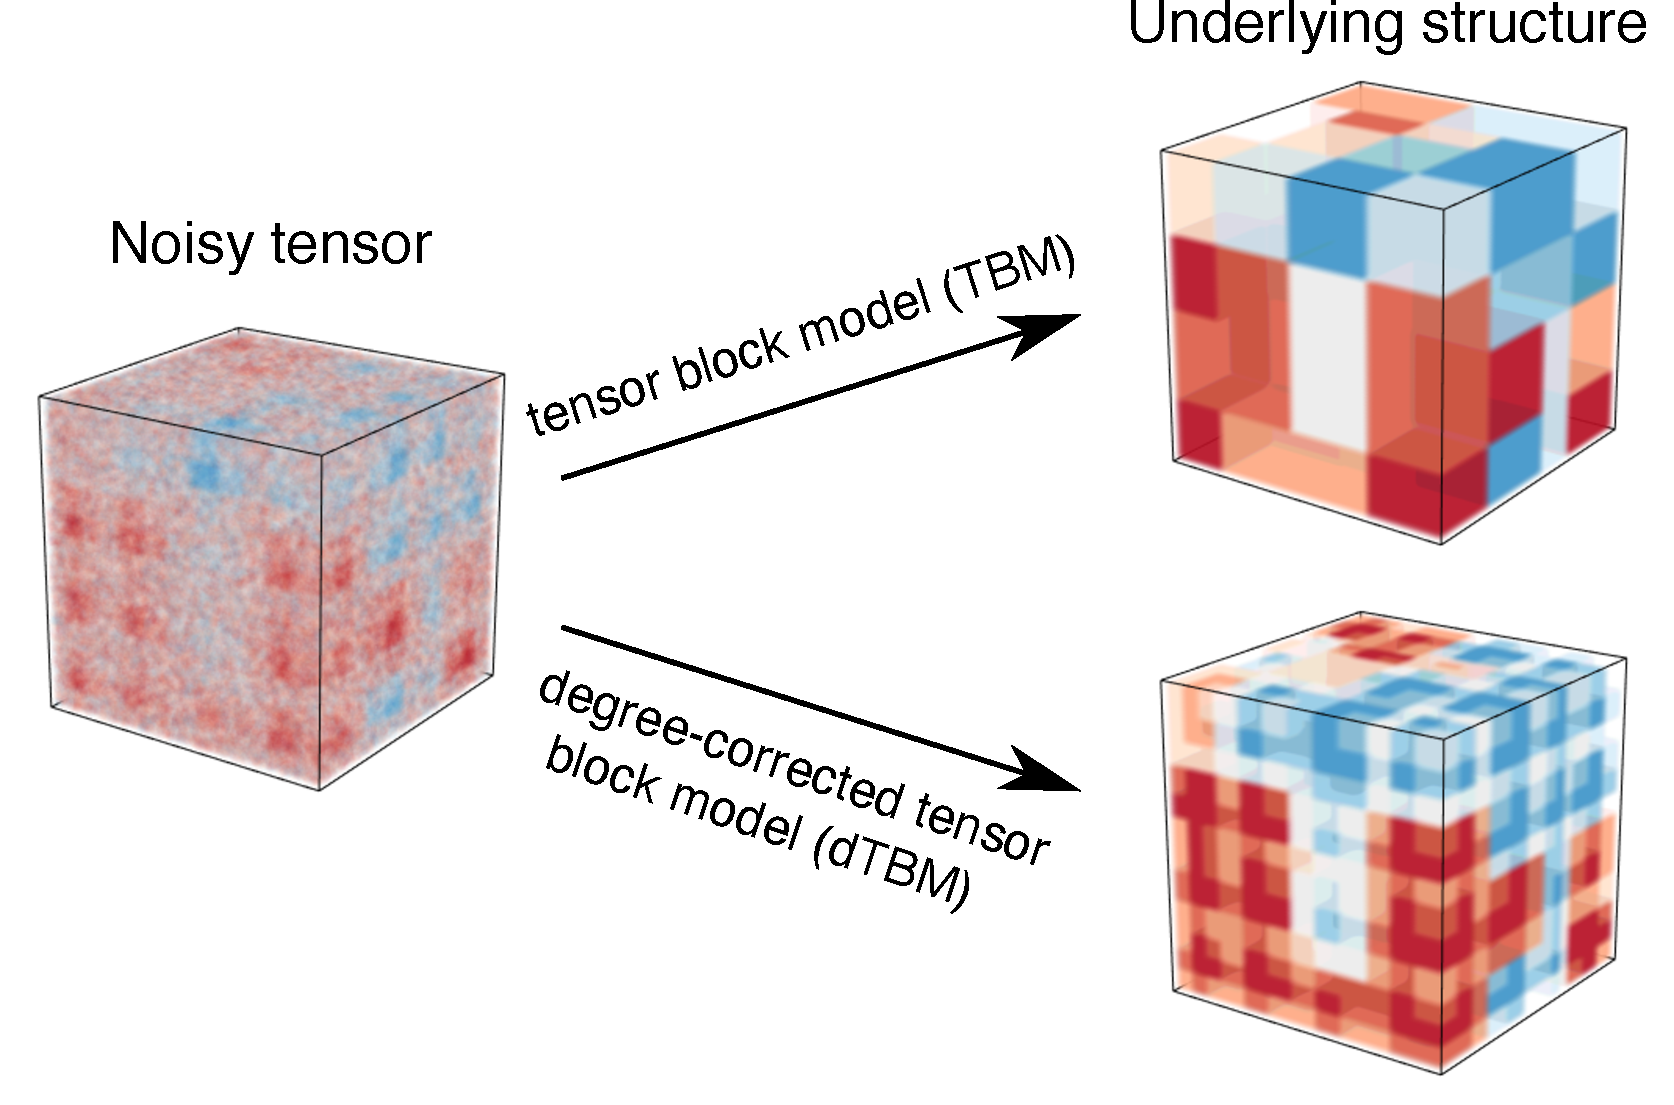
\includegraphics[width = 7cm]{intro2_2.pdf}
%DIFDELCMD <     %%%
%DIFDELCMD < \caption{%
{%DIFAUXCMD
%DIFDELCMD < \footnotesize %%%
\DIFdelFL{Examples for order-3 tensor block model (TBM) with and without degree correction. Both TBM and dTBM have four communities on each mode, while dTBM allows a richer structure with degree heterogeneity. }}
    %DIFAUXCMD
%DIFDELCMD < \label{fig:intro}
%DIFDELCMD <     \vspace{-.3cm}
%DIFDELCMD < \end{figure}
%DIFDELCMD < 

%DIFDELCMD < %%%
\DIFdel{We develop the }\DIFdelend \DIFaddbegin \DIFadd{The }\DIFaddend \emph{degree-corrected tensor block model} (dTBM) \DIFaddbegin \DIFadd{has been proposed recently }\DIFaddend to account for the degree heterogeneity\DIFaddbegin \DIFadd{~\mbox{%DIFAUXCMD
\citep{ke2019community}}\hspace{0pt}%DIFAUXCMD
}\DIFaddend . The dTBM combines a higher-order checkerboard structure with degree parameter \DIFdelbegin \DIFdel{$\mtheta=(\theta(1),\ldots,\theta(p))^T$ }\DIFdelend \DIFaddbegin \DIFadd{$\mtheta=(\mtheta(1),\ldots,\mtheta(p))^T$ }\DIFaddend to allow heterogeneity among $p$ nodes.  \DIFdelbegin \DIFdel{Fig.}\DIFdelend \DIFaddbegin \DIFadd{Figure}\DIFaddend ~\ref{fig:intro} compares the underlying structures of TBM and dTBM with the same number of communities. The dTBM allows varying values within the same community, thereby allowing a richer structure. \DIFaddbegin \DIFadd{To solve dTBM, we project clustering objects to a unit sphere and perform iterative clustering based on angle similarity. We refer to the algorithm as the }\textit{\DIFadd{spherical}} \DIFadd{clustering; detailed procedures are in Section~\ref{sec:alg}. The spherical clustering avoids the estimation of nuisance degree heterogeneity. The usage of angle similarity brings new challenges to the theoretical results, and we develop new polar-coordinate based techniques in the proofs. 
}\DIFaddend 


\DIFaddbegin \begin{figure}[t]
    \centering
    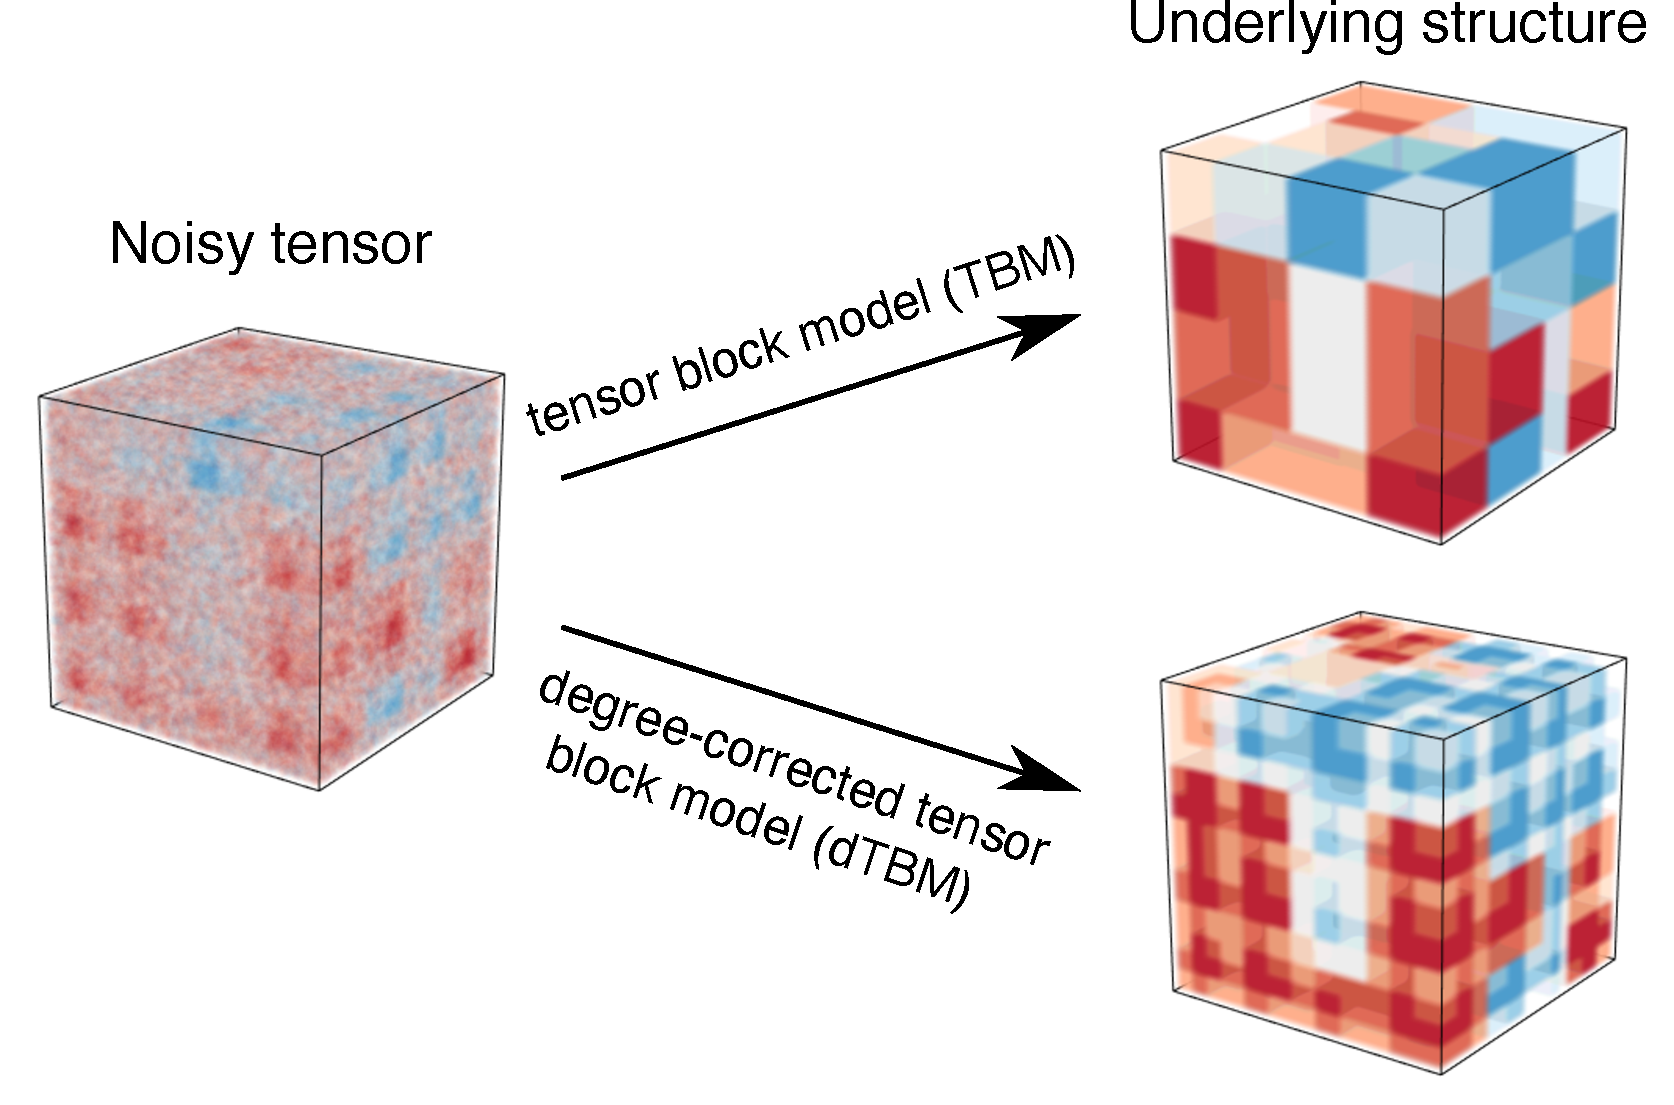
\includegraphics[width = .9\columnwidth]{intro2_2.pdf}
    \caption{ \small \DIFaddFL{Examples for order-3 TBM with and without degree correction. Both TBM and dTBM have four communities on each mode, while dTBM allows a richer structure with degree heterogeneity.
    }}
    \label{fig:intro}
\end{figure}

\DIFaddend {\bf Our contributions.} The primary goal of this paper is to provide both statistical and computational guarantees for dTBM. Our main contributions are summarized below.
\DIFdelbegin %DIFDELCMD < \begin{itemize}[wide,topsep=-2pt,itemsep=4pt,parsep=4pt]
%DIFDELCMD < %%%
\DIFdelend \DIFaddbegin \begin{itemize}[wide,topsep=-2pt,itemsep=2pt,parsep=4pt]
\DIFaddend 

 \item We develop a general dTBM and establish the identifiability for the uniqueness of clustering using the notion of angle \DIFdelbegin \DIFdel{seperability}\DIFdelend \DIFaddbegin \DIFadd{separability}\DIFaddend .

\item  We present the phase transition of clustering performance with respect to three different statistical and computational behaviors.  We characterize, for the first time, the critical signal-to-noise (SNR) thresholds in dTBMs, revealing the intrinsic distinctions \DIFdelbegin \DIFdel{between (}\DIFdelend \DIFaddbegin \DIFadd{among (vector) one-dimensional clustering, (}\DIFaddend matrix) biclustering\DIFaddbegin \DIFadd{, }\DIFaddend and (tensor) higher-order clustering. Specific SNR thresholds and algorithm \DIFdelbegin \DIFdel{behaviours }\DIFdelend \DIFaddbegin \DIFadd{behaviors }\DIFaddend are depicted in  \DIFdelbegin \DIFdel{Fig.}\DIFdelend \DIFaddbegin \DIFadd{Figure}\DIFaddend ~\ref{fig:phase_axis}. 

 \item We provide an angle-based algorithm that achieves exact clustering \emph{in polynomial time} under mild conditions. Simulation and data studies demonstrate the outperformance of our algorithm compared with existing higher-order clustering algorithms. 
\end{itemize}
The last two contributions, to our best knowledge, are new to the literature of dTBMs. 
%DIF < Table~\ref{tab:comp} highlights the improvement of our methods over previous results. Our algorithm addresses higher-order tensor data with degree heterogeneity, allows either binary or continuous entries, and achieves exponentially fast rate in misclustering error. 



\DIFdelbegin %DIFDELCMD < \begin{table*}[http]
%DIFDELCMD <     %%%
\DIFdelendFL \DIFaddbeginFL \begin{figure*}[t]
    \DIFaddendFL \centering
    \DIFdelbeginFL %DIFDELCMD < \begin{tabular}{c|ccccc}
%DIFDELCMD < \hline
%DIFDELCMD <     & {\small %%%
\DIFdelFL{Gao et al~\mbox{%DIFAUXCMD
\cite{gao2018community}}\hspace{0pt}%DIFAUXCMD
}%DIFDELCMD < }& {\small %%%
\DIFdelFL{Han et al~\mbox{%DIFAUXCMD
\cite{han2020exact}}\hspace{0pt}%DIFAUXCMD
}%DIFDELCMD < }& {\small %%%
\DIFdelFL{Ke et al~\mbox{%DIFAUXCMD
\cite{ke2019community}}\hspace{0pt}%DIFAUXCMD
}%DIFDELCMD < }& {\small %%%
\DIFdelFL{Ghoshdastidar et al~\mbox{%DIFAUXCMD
\cite{ghoshdastidar2017consistency}}\hspace{0pt}%DIFAUXCMD
}%DIFDELCMD < } &{\small %%%
\textbf{\DIFdelFL{Ours}}%DIFAUXCMD
%DIFDELCMD < }\\
%DIFDELCMD <     \hline
%DIFDELCMD <         {\small %%%
\DIFdelFL{Applicable to tensors}%DIFDELCMD < }& %%%
\DIFdelFL{$\times$ }%DIFDELCMD < & %%%
\DIFdelFL{$\surd$ }%DIFDELCMD < & %%%
\DIFdelFL{$\surd$ }%DIFDELCMD < &%%%
\DIFdelFL{$\surd$ }%DIFDELCMD < & %%%
\DIFdelFL{$\surd$  }%DIFDELCMD < \\
%DIFDELCMD <         {\small %%%
\DIFdelFL{Allow degree heterogeneity}%DIFDELCMD < } &  %%%
\DIFdelFL{$\surd$ }%DIFDELCMD < & %%%
\DIFdelFL{$\times$ }%DIFDELCMD < & %%%
\DIFdelFL{$\surd$ }%DIFDELCMD < &%%%
\DIFdelFL{$\surd$ }%DIFDELCMD < & %%%
\DIFdelFL{$\surd$ }%DIFDELCMD < \\
%DIFDELCMD <         %%%
%DIF < Assortative assumption&  $\surd$ & $\times$ & $\times$ & $\times$\\
       %DIFDELCMD < {\small %%%
\DIFdelFL{Allow various data types}%DIFDELCMD < } & %%%
\DIFdelFL{$\times$ }%DIFDELCMD < & %%%
\DIFdelFL{$\surd$ }%DIFDELCMD < & %%%
\DIFdelFL{$\times$ }%DIFDELCMD < & %%%
\DIFdelFL{$\surd$  }%DIFDELCMD < &%%%
\DIFdelFL{$\surd$}%DIFDELCMD < \\
%DIFDELCMD <         {\small %%%
\DIFdelFL{Misclustering rate (for order 2)}%DIFDELCMD < }& %%%
\DIFdelFL{$\exp(-p)$ }%DIFDELCMD < & %%%
\DIFdelFL{$\exp(-p)$ }%DIFDELCMD < & %%%
\DIFdelFL{$p^{-1}$ }%DIFDELCMD < & %%%
\DIFdelFL{$p^{-1}$}%DIFDELCMD < & %%%
\DIFdelFL{$\exp(-p)$}%DIFDELCMD < \\
%DIFDELCMD <         \hline
%DIFDELCMD <     \end{tabular}
%DIFDELCMD <     %%%
%DIFDELCMD < \caption{%
{%DIFAUXCMD
\DIFdelFL{Comparison between previous methods with our method. }}%DIFAUXCMD
%DIFDELCMD < \label{tab:comp}
%DIFDELCMD < \end{table*}
%DIFDELCMD < 

%DIFDELCMD < \begin{figure*}[http]
%DIFDELCMD <     \centering
%DIFDELCMD <     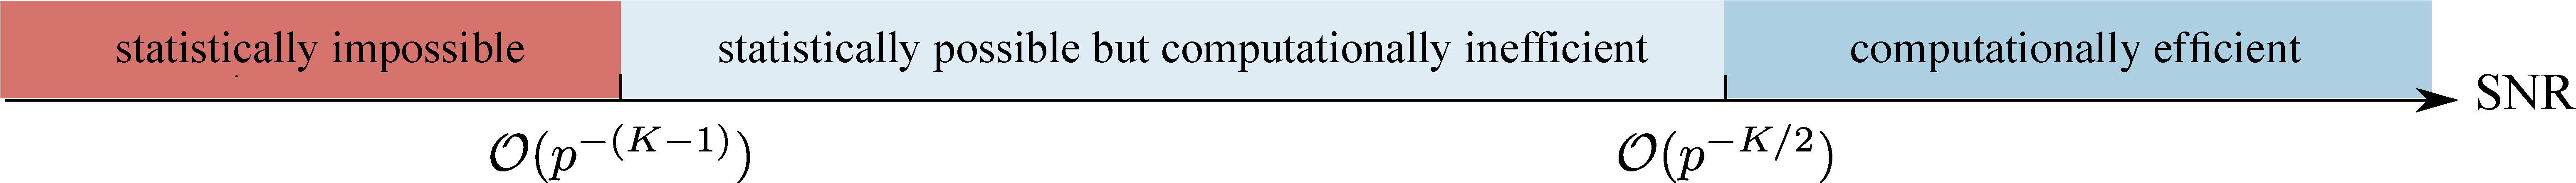
\includegraphics[width = 17cm]{phase.pdf}
%DIFDELCMD <     %%%
\DIFdelendFL \DIFaddbeginFL 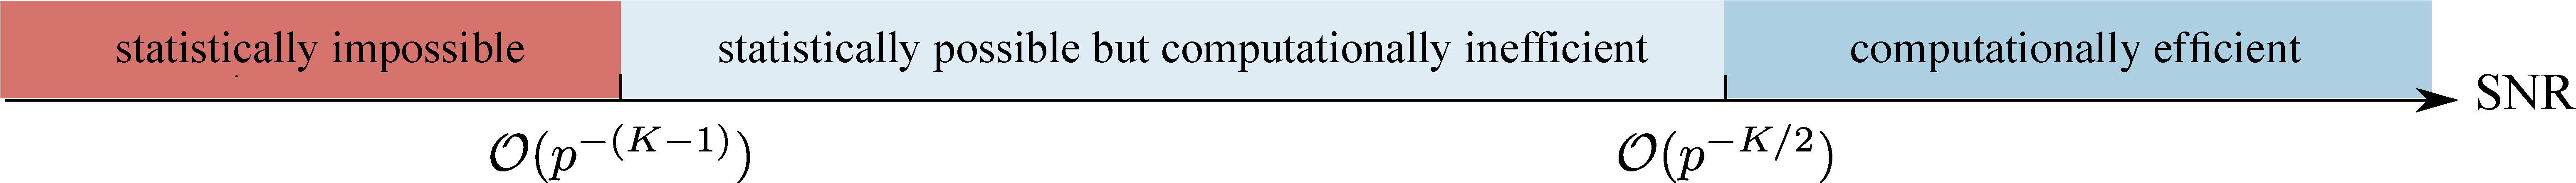
\includegraphics[width = .9\textwidth]{phase.pdf}
    \DIFaddendFL \caption{\DIFdelbeginFL %DIFDELCMD < \footnotesize %%%
\DIFdelendFL  \DIFaddbeginFL \small \DIFaddendFL SNR thresholds for statistical and computational limits in order-$K$ dTBM with dimension $(p,...,p)$ \DIFaddbeginFL \DIFaddFL{and $K \geq 2$}\DIFaddendFL . The SNR gap between statistical possibility and computational efficiency  exists only for tensors with $K \geq 3$. }
    \label{fig:phase_axis}
\end{figure*}


\DIFaddbegin \thispagestyle{empty}

\DIFaddend {\bf Related work.} 
%DIF < Our work is closely related to, but also distinct from several lines of existing research. 
\DIFdelbegin \DIFdel{We emphasize the comparisons that set our work apart from earlier literature from two perspectives---models and algorithms. From the model perspective, our work extends the previous }\DIFdelend \DIFaddbegin \DIFadd{Our work is closely related to but also distinct from several lines of existing research. Table~\ref{tab:comp} summarizes the most relevant models. 
    }

    \textit{\DIFadd{Block model.}} \DIFadd{Block models such as stochastic block model (SBM) and }\DIFaddend degree-corrected \DIFdelbegin \DIFdel{model from matrices to tensors. There is a huge literature on degree-corrected matrix models; see }\DIFdelend \DIFaddbegin \DIFadd{SBM have been widely used for matrix clustering problems. See }\DIFaddend the review paper~\DIFdelbegin \DIFdel{\mbox{%DIFAUXCMD
\cite{abbe2017community} }\hspace{0pt}%DIFAUXCMD
}\DIFdelend \DIFaddbegin \DIFadd{\mbox{%DIFAUXCMD
\citep{abbe2017community} }\hspace{0pt}%DIFAUXCMD
}\DIFaddend and the references therein.
    \DIFdelbegin \DIFdel{The tensor counterparts, however, are relatively less understood. Tab. ~\ref{tab:comp} summarizes  the most relevant models for }\DIFdelend %DIF > However, The tensor counterparts are relatively less understood.  
    \DIFaddbegin \DIFadd{The (non-degree) tensor block model (TBM) is a }\DIFaddend higher-order \DIFdelbegin \DIFdel{clustering. Earlier tensor methods either fail to allow degree heterogeneity~\mbox{%DIFAUXCMD
}\hspace{0pt}%DIFAUXCMD
, or suffer from sub-optimal misclustering rates ~\mbox{%DIFAUXCMD
\cite{ke2019community,ghoshdastidar2017consistency,chi2020provable}}\hspace{0pt}%DIFAUXCMD
. In contrast, our method addresses the degree heterogeneity, allows discrete and continuous entries, and achieves exponentially fast rate in clustering tasks. }\DIFdelend \DIFaddbegin \DIFadd{extension of SBM, and its statistical-computational properties are investigated in recent literatures~\mbox{%DIFAUXCMD
\citep{wang2019multiway, han2020exact, ghoshdastidar2017consistency}}\hspace{0pt}%DIFAUXCMD
. Extending results from non-degree to degree-corrected model is highly challenging. Our dTBM parameter space is equipped with angle-based similarity and nuisance degree parameters. The extra complexity makes the Cartesian coordinates based analysis~\mbox{%DIFAUXCMD
\citep{han2020exact} }\hspace{0pt}%DIFAUXCMD
non-applicable to our setting. Towards this goal, we have developed a new polar coordinates based analysis to control the model complexity. We also develop a new angle-based iteration algorithm to achieve optimal clustering rates }\emph{\DIFadd{without the need of estimating nuisance degree parameters}}\DIFadd{.
    }\DIFaddend 

     \DIFdelbegin \DIFdel{From the algorithm perspective, our }\DIFdelend \DIFaddbegin \textit{\DIFadd{Degree-corrected block model.}} \DIFadd{The hypergraph degree-corrected block model (hDCBM) and its variant have been proposed in the literature~\mbox{%DIFAUXCMD
\citep{ke2019community, yuan2018testing}}\hspace{0pt}%DIFAUXCMD
. For this popular model, however, the optimal statistical-computational rates remain an open problem. Our main contribution is to provide a sharp statistical and computational critical phase transition in dTBM literature. In addition, our algorithm results in a faster }\emph{\DIFadd{exponential}} \DIFadd{error rate, in contrast to the }\emph{\DIFadd{polynomial}} \DIFadd{rate in~\mbox{%DIFAUXCMD
\cite{ke2019community}}\hspace{0pt}%DIFAUXCMD
. The original hDCBM~\mbox{%DIFAUXCMD
\citep{ke2019community} }\hspace{0pt}%DIFAUXCMD
is designed for binary observations only, and we extend the model to both continuous and binary observations. We believe our results are novel and helpful to the community. See Figure~\ref{fig:phase_axis} for overview of our results. 
    }

    \textit{\DIFadd{Global-to-local algorithm strategy.}} \DIFadd{Our }\DIFaddend methods generalize the recent global-to-local strategy for matrix learning~\citep{gao2018community,chi2019nonconvex,yun2016optimal}  to tensors~\citep{han2020exact,ahn2018hypergraph,kim2018stochastic}. Despite the conceptual similarity, we address several fundamental challenges associated with this non-convex, non-continuous problem. We show the insufficiency of the conventional tensor HOSVD~\DIFdelbegin \DIFdel{\mbox{%DIFAUXCMD
\cite{kolda2009tensor}}\hspace{0pt}%DIFAUXCMD
}\DIFdelend \DIFaddbegin \DIFadd{\mbox{%DIFAUXCMD
\citep{de2000multilinear}}\hspace{0pt}%DIFAUXCMD
}\DIFaddend , and we develop a weighted higher-order initialization that relaxes the \DIFdelbegin \DIFdel{eigen-gap }\DIFdelend \DIFaddbegin \DIFadd{singular-value gap }\DIFaddend separation condition. Furthermore, our local iteration leverages the angle-based clustering in order to avoid explicit estimation of degree heterogeneity. Our bounds reveal the interesting interplay between the computational and statistical errors. We show that our final estimate \DIFdelbegin \DIFdel{provably }\DIFdelend \DIFaddbegin \emph{\DIFadd{provably}} \DIFaddend achieves the exact clustering within only polynomial-time complexity. 




\DIFaddbegin \begin{table*}[t]
\resizebox{\textwidth}{!}{%
\centering
    \begin{tabular}{c|ccccc}
\hline
    & \cite{gao2018community}&  \cite{han2020exact}&  \cite{ghoshdastidar2017consistency} &\cite{ke2019community} & \textbf{Ours}\\
    \hline
      Allow tensors of arbitrary order & $\times$ & $\surd$ & $\surd$ &$\surd$ & $\surd$  \\
        Allow degree heterogeneity &  $\surd$ & $\times$ & $\surd$ &$\surd$ & $\surd$ \\
        Singular-value gap-free clustering &  $\surd$ & $\surd$ & $\times$ & $\times$ &$\surd$ \\
        Misclustering rate (for order $K^*$)& - & $\exp(-p^{K/2})$ & $p^{-1}$& $p^{-2}$ &  $\exp(-p^{K/2})$\\
        \hline
    \end{tabular}
    }
    \caption{\small \DIFaddFL{Comparison between previous methods with our method. $^*$We list the result for order-K tensors with $K \geq 3$ and general number of communities $r = \tO(1)$. }}\label{tab:comp}
    \vspace{-.2cm}
\end{table*}
\thispagestyle{empty}

\DIFaddend {\bf Notation.} We use lower-case letters (e.g., \DIFdelbegin \DIFdel{$a,\theta$}\DIFdelend \DIFaddbegin \DIFadd{$a,b$}\DIFaddend ) for scalars, lower-case boldface letters (e.g., $\ma,\mtheta$) for vectors, upper-case boldface letters (e.g., $\mX,\mY$) for matrices, and calligraphy letters (e.g., $\tX,\tY$) for tensors of order three or greater. We use \DIFaddbegin \DIFadd{$\mone_p$ to denote a vector of length $p$ with all entries to be 1. We use }\DIFaddend $|\cdot|$ for the cardinality of a set and $\ind\{\cdot\}$ for the indicator function. For an integer $p\in\mathbb{N}_{+}$, we use the shorthand $[p]= \offf{1,2,...,p}$. For a \DIFaddbegin \DIFadd{length-}\DIFaddend $p$ \DIFdelbegin \DIFdel{-length vector $\ma = (a_1,\ldots,a_p)$}\DIFdelend \DIFaddbegin \DIFadd{vector $\ma$}\DIFaddend , we use \DIFaddbegin \DIFadd{$a(i)\in\mathbb{R}$ to denote the $i$-th entry of $\ma$, and use }\DIFaddend $\ma_{I}$ to denote the sub-vector by restricting the indices in the set $I\subset [p]$.  We use  \DIFdelbegin \DIFdel{$\onorm{\ma}=(\sum_{i}a^2_i)^{1/2}$ }\DIFdelend \DIFaddbegin \DIFadd{$\onorm{\ma}=\sqrt{\sum_{i}a^2(i)}$ }\DIFaddend to denote the $\ell_2$-norm, $\onorm{\ma}_1=\sum_i |a_i|$ to denote the $\ell_1$ norm of $\ma$. For \DIFdelbegin \DIFdel{a matrix $\mY$, we use $\mY_{i:}$ to  denote the $i$-th row of the matrix. We let $\tY = \entry{\tY(i_1,\ldots,i_K)} \in \bbR^{p_1 \times \cdots \times p_K}$ }\DIFdelend \DIFaddbegin \DIFadd{two vector $\ma, \mb$ of the same dimension, we }\DIFaddend denote \DIFaddbegin \DIFadd{the angle between $\ma, \mb$ by $\cos \of{\ma, \mb} = \ang{ \ma, \mb} / \onorm{\ma} \onorm{\mb},$ where $\ang{\ma,\mb}$ is the inner product of two vectors and $\cos \of{\ma, \mb} \in [-1,1]$. We make the convention that $\cos \of{\ma, \mb} = \cos \of{\ma^T, \mb^T}$. Let $\tY  \in \bbR^{p_1 \times \cdots \times p_K}$ be }\DIFaddend an order-$K$ $(p_1,...,p_K)$-dimensional tensor. \DIFaddbegin \DIFadd{We use $\tY(i_1,\ldots,i_K)$ to denote the $(i_1,\ldots,i_K)$-th entry of $\tY$. }\DIFaddend The multilinear multiplication of a tensor $\tS\in \bbR^{r_1\times \cdots \times r_K}$ by matrices $\mM_k \in\mathbb{R}^{p_k\times r_k}$ results in an order-$d$ $(p_1,\ldots,p_K)$-dimensional tensor $\tX$
\DIFdelbegin \DIFdel{, denoted
}\DIFdelend \[
\tX=\tS \times_1 \mM_1 \times \cdots \times_K \mM_K,
\]
where the entries of $\tX$ are defined by \DIFdelbegin \begin{align*}
    &\DIFdel{\tX(i_1,\ldots, i_K)}\\ &\DIFdel{=\sum_{(j_1,\ldots,j_K)}\tS(j_1,\ldots,j_K)\mM_1(i_1,j_1)\cdots \mM_K(i_K,j_K).
}\end{align*}%DIFAUXCMD
%DIFDELCMD < 

%DIFDELCMD <  %%%
\DIFdelend \DIFaddbegin \DIFadd{$\tX(i_1,\ldots, i_K)
    =\sum_{(j_1,\ldots,j_K)}\tS(j_1,\ldots,j_K)\mM_1(i_1,j_1)\cdots \mM_K(i_K,j_K).$
%DIF >  \small
%DIF >  \begin{align}
%DIF >      &\tX(i_1,\ldots, i_K)\\
%DIF >      &=\sum_{(j_1,\ldots,j_K)}\tS(j_1,\ldots,j_K)\mM_1(i_1,j_1)\cdots \mM_K(i_K,j_K).
%DIF >  \end{align} 
%DIF >  \normalsize
For a matrix $\mY$, we use $\mY_{i:}$ (respectively, $\mY_{:i}$) to denote the $i$-th row (respectively, $i$-th column) of the matrix. Similarly, for an order-3 tensor, we use $\tY_{::i}$ to denote the $i$-th matrix slide of the tensor. }\DIFaddend We use $\text{Ave}(\cdot)$ to denote the operation of taking averages across elements and $\text{Mat}_k(\cdot)$ to denote the unfolding operation that reshapes the tensor along mode $k$ into a matrix. For a symmetric tensor $\tY\in\mathbb{R}^{p\times \cdots \times p}$, we omit the subscript and use $\text{Mat}(\tY)\in\mathbb{R}^{p\times p^{K-1}}$ to denote the unfolding. For two sequences $\{a_p\}, \{b_p\}$, we denote $a_p\lesssim b_p$ \DIFaddbegin \DIFadd{or $a_p=\tO(b_p)$ if $\lim_{p\to\infty}a_p /b_p\leq c$ for some constant $c\geq 0$, $a_p=o(b_p)$ }\DIFaddend if \DIFdelbegin \DIFdel{$\lim_{p\to\infty} a_p/b_p \leq c$ }\DIFdelend \DIFaddbegin \DIFadd{$\lim_{p\to\infty}a_p/b_p =0$, }\DIFaddend and $a_p = \Omega(b_p)$ if \DIFdelbegin \DIFdel{$c b_p \leq a_p \leq C b_p$, for some constants $c, C\geq 0$}\DIFdelend \DIFaddbegin \DIFadd{both $b_p \lesssim a_p$ and $a_p\lesssim b_p$}\DIFaddend . Throughout the paper, we use the terms ``community'' and ``clusters'' exchangeably. 
\DIFdelbegin %DIFDELCMD < \fixme{Miaoyan}{\color{red} need to define $\cos(\ma,\mb)$. Be careful with signs.}
%DIFDELCMD < %%%
\DIFdelend 


\DIFdelbegin %DIFDELCMD < \vspace{-.05cm}
%DIFDELCMD < %%%
\DIFdelend %DIF >  {\bf Organization.} The rest of this paper is organized as follows. Section~\ref{sec:model} introduces the degree-corrected tensor block model (dTBM) with three motivating examples and presents the identifiability of dTBM under the angle gap condition. We show the phase transition and the existence of statistical-computational gaps for the higher-order dTBM in Section~\ref{sec:limits}. In Section~\ref{sec:alg}, we provide a polynomial-time two-stage algorithm with misclustering rate guarantees. Numerical studies including the simulation, comparison with other methods, and two real dataset analyses are in Sections~\ref{sec:simulation}-\ref{sec:real}. The main technical ideas we develop for addressing main theorems are provided in Section~\ref{sec:mainproof}. Detailed proofs and extra theoretical results are provided in Appendix.
\DIFaddbegin 


\DIFaddend \section{\DIFdelbegin \DIFdel{Model formulation}\DIFdelend \DIFaddbegin \DIFadd{MODEL FORMULATION}\DIFaddend }\label{sec:model}

\subsection{\DIFdelbegin \DIFdel{Degree-corrected tensor block model}\DIFdelend \DIFaddbegin \DIFadd{dTBM}\DIFaddend }

Suppose we have an order-$K$ data tensor $\tY \in \bbR^{p \times \cdots \times p}$. For ease of notation, we focus on symmetric tensors in this section\DIFdelbegin \DIFdel{; our framework easily extends to general asymmetric tensors}\DIFdelend . Assume there exist $r \geq 2$  disjoint communities among the $p$ nodes. We represent the community assignment by a function $z \colon [p]\mapsto[r]$, where $z(i) = a$ for $i$-th node that belongs to the $a$-th community. Then, $z^{-1}(a)=\{i\in[p]\colon z(i)=a\}$ denotes the set of nodes that belong to the $a$-th community, and $|z^{-1}(a)|$ denotes the number of nodes in the $a$-th community. %DIF < , and we let $p_a = \sum_{i \in [p]}\ind \offf{ z_i= a}$ denote the size of $a$-th community. 
Let $\mtheta=(\theta(1),\ldots,\theta(p))^T$ denote the degree heterogeneity for $p$ nodes. We consider the order-$K$ dTBM~\DIFdelbegin \DIFdel{\mbox{%DIFAUXCMD
\cite{ghoshdastidar2017consistency,ke2019community}}\hspace{0pt}%DIFAUXCMD
,
}%DIFDELCMD < 

%DIFDELCMD < \vspace{-.7cm}
%DIFDELCMD < %%%
\DIFdelend \DIFaddbegin \DIFadd{\mbox{%DIFAUXCMD
\citep{ke2019community}}\hspace{0pt}%DIFAUXCMD
,
}\vspace{-0.2cm}
\footnotesize
\DIFaddend \begin{equation}\label{eq:model_margin}
    \DIFdelbegin %DIFDELCMD < \footnotesize
%DIFDELCMD <     %%%
\DIFdelend \tY(i_1,\ldots,i_K) = \tS(z(i_1),\ldots,z(i_K)) \prod_{k = 1}^K\theta_{i_k} + \tE(i_1,\ldots,i_K), 
\end{equation}
\normalsize
where $\tS \in \bbR^{r \times \cdots \times r}$ is an order-$K$ tensor collecting the block means among communities, and $\tE\in\mathbb{R}^{p\times \cdots \times p}$ is a noise tensor consisting of independent \DIFdelbegin \DIFdel{mean-zero }\DIFdelend \DIFaddbegin \DIFadd{zero-mean }\DIFaddend sub-Gaussian entries with variance bounded by $\sigma^2$. The unknown parameters are $z$, $S$, and $\mtheta$. The dTBM can be equivalently written in a compact form of tensor-matrix product:
\begin{equation}\label{eq:model_tensor}
\DIFdelbegin \DIFdel{\mathbb{E}}\DIFdelend \DIFaddbegin \bbE\DIFaddend \tY = \tS \times_1 \mTheta \mM \times_2 \cdots \times_K  \mTheta \mM,
\end{equation}
where $\mTheta = \text{diag}(\theta(1),...,\theta(p)) \in \bbR^{p \times p}$ is a diagonal matrix, $\mM \in \offf{0,1}^{p \times r}$ is the membership matrix associated with community assignment $z$ such that $\mM(i,j)=\ind\{z(i)=j\}$. By definition, each row of $\mM$ has one copy of 1's and 0's elsewhere. Note that the discrete nature of $\mM$ renders our model~\eqref{eq:model_tensor} more challenging than Tucker decomposition. %DIF < The Tucker rank of the signal tensor $\bbE \tY$ is bounded by, but not necessarily equal to, $(r,...,r)$~\cite{wang2019multiway}. 
We call a tensor \DIFdelbegin \DIFdel{$\tX$ }\DIFdelend \DIFaddbegin \DIFadd{$\tY$ }\DIFaddend an $r$-block tensor with degree $\mtheta$ %DIF < with the core tensor $\tS$ 
\DIFdelbegin \DIFdel{if $\tX$ admitsdTBM}\DIFdelend \DIFaddbegin \DIFadd{if $\tY$ admits}\DIFaddend ~\eqref{eq:model_tensor}. 
%DIF > The goal of clustering is to estimate $z$ from a single noisy tensor $\tY$. 
\DIFaddbegin \DIFadd{We are particularly interested in high-dimensional regime where $p$ grows whereas $r=\tO(1)$.   The extension to general asymmetrical dTBM is obtained via replacing $(\mM, \mTheta)$ in~}\eqref{eq:model_tensor} \DIFadd{by mode-specific parameters $(\mM_k, \mTheta_k)$ for every mode $k\in[K]$. }\DIFaddend Here, we give two special cases of dTBM.
\DIFaddbegin 

\DIFaddend \begin{example}[Gaussian TBM]
Let $\theta(i)= 1$ for all $i \in [p]$ and $\tE$ be a noise tensor with i.i.d.\ $N(0,\sigma^2)$ entries. Our dTBM reduces to a non-degree Gaussian TBM~\citep{wang2019multiway, han2020exact}, which is widely used in previous clustering algorithms~\DIFdelbegin \DIFdel{\mbox{%DIFAUXCMD
\cite{wang2019multiway,chi2020provable}}\hspace{0pt}%DIFAUXCMD
. 
The theoretical results in TBM serve as benchmarks for dTBM. 
}\DIFdelend \DIFaddbegin \DIFadd{\mbox{%DIFAUXCMD
\citep{wang2019multiway,chi2020provable}}\hspace{0pt}%DIFAUXCMD
. 
%DIF > The theoretical results in TBM serve as benchmarks for dTBM. 
}\DIFaddend \end{example}

\begin{example}[Binary dTBM]
Consider a $K$-uniform hypergraph $H = (V,E)$, where $V = [p]$ collects the nodes with $r$ disjoint communities and $E$ collects all the $K$-way hyperedges. Let $\tY \in \{0,1\}^{p \times \cdots \times p}$ denote the adjacency tensor, where the entries encode the presence or absence of hyperdeges among $p$ nodes. Specifically, let $\tY(i_1,...,i_K) = 1$ if  $(i_1,...,i_K) \in E$, otherwise, $\tY(i_1,...,i_K) = 0$, for all $(i_1,\ldots,i_K) \in [p]^K$. The equation~\eqref{eq:model_tensor} models $\mathbb{E}\tY$ with \DIFdelbegin \DIFdel{unknown }\DIFdelend degree heterogeneity and subgaussianity parameter $\sigma^2 = 1/4$. 
\end{example}




\DIFdelbegin %DIFDELCMD < \begin{rmk}[Comparison with non-degree models]
%DIFDELCMD < %%%
\DIFdel{Our dTBM uses fewer block parameters than TBM. Let the subscripts ``deg" and ``non" denote quantities in the models with and without degrees, respectively. Then, every $r_{\text{non}}$-block tensor can be represented by a degree-corrected $r_{\text{deg}}$-block tensor with $r_{\text{deg}}\leq r_{\text{non}}$. In particular, there exist tensors with $r_{\text{non}}=p$ but $r_{\text{deg}}=1$, so the reduction in $r$ can be dramatic from $p$ to 1. This fact highlights the benefits of introducing degree heterogeneity in higher-order clustering tasks.
}%DIFDELCMD < \end{rmk}
%DIFDELCMD < %%%
\DIFdelend %DIF >  \begin{rmk}[Comparison with non-degree models]
%DIF >  Our dTBM uses fewer block parameters than TBM. In particular, every non-degree $r_1$-block tensor can be represented by a \emph{degree-corrected} $r_2$-block tensor with $r_2\leq r_1$. In particular, there exist tensors with $r_1=p$ but $r_2=1$, so the reduction in model complexity can be dramatic from $p$ to 1. This fact highlights the benefits of introducing degree heterogeneity in higher-order clustering tasks.
%DIF >  \end{rmk}


%DIF <  In addition, the following example highlights the benefits of degree correction in clustering tasks. 
%DIF <  \begin{example}[Comparison to non-degree models]\label{ex:benefit}
%DIF <  Every $r_{\text{non}}$-block tensor can be represented by degree-corrected $r_{\text{deg}}$-block tensor with $r_{\text{deg}}\leq r_{\text{non}}$. In particular, there exist tensors with $r_{\text{non}}=p$ but $r_{\text{deg}}=1$.
%DIF <  \end{example}
%DIF <  %In principle, every $(p,\ldots,p)$-dimensional tensor can be represented by a $p$-block tensor.
%DIF <  The above example shows that our dTBM uses fewer block parameters than TBM, and the reduction in $r$ can be dramatic from $p$ to 1. This fact shows the advantages of introducing degree heterogeneity in high-dimensional clustering.
\DIFdelbegin %DIFDELCMD < 

%DIFDELCMD < %%%
\DIFdelend \subsection{Identifiability under \DIFdelbegin \DIFdel{angle gap condition}\DIFdelend \DIFaddbegin \DIFadd{Angle Gap}\DIFaddend }
The goal of clustering is to estimate the partition function $z$ from model~\eqref{eq:model_tensor}. \DIFaddbegin \DIFadd{For ease of notation, we focus on symmetric tensors; the extension to non-symmetric tensors are similar. }\DIFaddend We use $\tP$ to denote the following parameter space for $(z,\tS,\mtheta)$,
\DIFdelbegin %DIFDELCMD < 

%DIFDELCMD < \vspace{-.3cm}
%DIFDELCMD < \small
%DIFDELCMD < %%%
\DIFdelend \DIFaddbegin \footnotesize
\DIFaddend \begin{align}\label{eq:family}
&\tP=\bigg\{(z,\tS,\mtheta)\colon  \DIFdelbegin \DIFdel{\ }\DIFdelend \mtheta\in\mathbb{R}^p_{+},\DIFdelbegin \DIFdel{\ 
}\DIFdelend \DIFaddbegin \DIFadd{\text{for }a\in[r], 
}\DIFaddend {c_1p\over r}\leq |z^{-1}(a)|\leq {c_2 p\over r},\notag \\
&c_3\leq \onormSize{}{\text{Mat}(\tS)_{a:}}\leq c_4,
\onorm{\mtheta_{z^{-1}(a)}}_1=|z^{-1}(a)| \DIFdelbegin \DIFdel{, a\in[r]}\DIFdelend \bigg\},
\DIFdelbegin \DIFdel{\ \ 
%DIF < & \text{for all }a\in[r] \text{ and }\min_{i\in[p]}\theta(i) \geq c_5>0 \bigg\},
}\DIFdelend \end{align}
\normalsize 
where $c_i>0$'s are universal constants. %DIF < We briefly describe the rationale of the constraints in~\eqref{eq:family}. 
\DIFaddbegin \DIFadd{We briefly describe the rationale of the constraints in~}\eqref{eq:family}\DIFadd{. 
}\DIFaddend First, the entrywise positivity constraint on  $\mtheta\in\mathbb{R}^p_{+}$ is imposed to avoid sign ambiguity between entries in $\mtheta_{z^{-1}(a)}$ and $\tS$. This constraint \DIFaddbegin \DIFadd{allows the trigonometric $\cos$ to describe the angle similarity in the Assumption~\ref{assmp:min_gap} below and Sub-algorithm~}\hyperref[alg:main]{2} \DIFadd{in Section~\ref{sec:alg}. Note that the positivity constraint }\DIFaddend can be achieved without sacrificing model flexibility, by using a slightly larger dimension of $\tS$ in the factorization~\eqref{eq:model_tensor}\DIFdelbegin \DIFdel{(see Supplement)}\DIFdelend \DIFaddbegin \DIFadd{; see Supplement~\ref{subsec:positive}}\DIFaddend . Second, %DIF < the quantity $|z^{-1}(a)|$ denotes the number of nodes in $a$-th community. T
\DIFdelbegin \DIFdel{the }\DIFdelend \DIFaddbegin \DIFadd{recall that the quantity $|z^{-1}(a)|$ denotes the number of nodes in $a$-th community. The }\DIFaddend constants $c_1, c_2$ in the $|z^{-1}(a)|$ bound assume the roughly balanced size across $r$ communities. Third, the constants $c_3, c_4 $ in the magnitude of $\text{Mat}(\tS)_{a:}$ requires no purely zero slide in $\tS$, so the core tensor $\tS$ is not trivially reduced to \DIFaddbegin \DIFadd{a }\DIFaddend lower rank. Lastly, the $\ell_1$ normalization $\onormSize{}{\mtheta_{z^{-1}(a)}}_1=|z^{-1}(a)|$ is imposed to avoid the scalar ambiguity between $\mtheta_{z^{-1}(a)}$ and $\tS$. This constraint, again, incurs no restriction to model flexibility but makes our presentation cleaner. \DIFaddbegin \DIFadd{See Supplement~\ref{subsec:comp_para} for the parameter space comparison with previous works.
}\DIFaddend 



We \DIFdelbegin \DIFdel{first provide the identifiablity }\DIFdelend \DIFaddbegin \DIFadd{now provide the identifiability }\DIFaddend conditions for our model before estimation procedures. When $r=1$, the decomposition~\eqref{eq:model_tensor} is always unique (up to cluster label permutation) in $\tP$, because dTBM is equivalent to the rank-1 tensor family under this case. When $r\geq 2$, the Tucker rank of signal tensor \DIFdelbegin \DIFdel{$\mathbb{E}\tY$ }\DIFdelend \DIFaddbegin \DIFadd{$\bbE\tY$ }\DIFaddend in~\eqref{eq:model_tensor} is bounded by, but not necessarily equal to, the number of blocks $r$~\citep{wang2019multiway}. Therefore, one can not apply the classical identifiability conditions for low-rank tensors to dTBM. Here, we introduce a key separation condition on the core tensor. 

\begin{assumption}[Angle gap] \label{assmp:min_gap}Let $\mS = \text{Mat}(\tS)$. Assume the minimal gap between normalized rows of $\mS$ is bounded away from zero\DIFdelbegin \DIFdel{, }\DIFdelend \DIFaddbegin \DIFadd{; }\DIFaddend i.e., \DIFaddbegin \DIFadd{for $r \geq 2$,
}\DIFaddend \begin{equation}\label{eq:minimal_gap}
    \Delta_{\min} := \min_{a \neq b \in [r]} \onorm{\frac{\mS_{a:}}{\onormSize{}{ \mS_{a:}}} - \frac{\mS_{b:}}{\onormSize{}{ \mS_{b:}}} }>0.
\end{equation}
\DIFdelbegin \DIFdel{Equivalently, }\DIFdelend \DIFaddbegin \end{assumption}
\DIFadd{We make the convention $\Delta_{\min} = 1$ for $r = 1$. Equivalently, }\eqref{eq:minimal_gap} \DIFadd{says that }\DIFaddend none of the two rows in $\mS$ are parallel\DIFdelbegin \DIFdel{, }\DIFdelend \DIFaddbegin \DIFadd{; }\DIFaddend i.e., \DIFdelbegin \DIFdel{$ \max_{a \neq b\in [r]}\cos \of{\mS_{a:},\  \mS_{b:}}  = 1-\Delta^2_{\min}/2<1$. }%DIFDELCMD < \end{assumption}
%DIFDELCMD < %%%
\DIFdelend \DIFaddbegin \DIFadd{$\max_{a \neq b\in [r]}\cos \of{\mS_{a:},\  \mS_{b:}}  = 1-\Delta^2_{\min}/2<1$. }\DIFaddend The quantity $\Delta_{\min}$ characterizes the non-redundancy among clusters measured by angle separation. \DIFdelbegin \DIFdel{The }\DIFdelend \DIFaddbegin \DIFadd{Denominators involved in }\DIFaddend definition~\eqref{eq:minimal_gap} \DIFdelbegin \DIFdel{is }\DIFdelend \DIFaddbegin \DIFadd{are }\DIFaddend well posed because of the lower bound on $\onorm{\mS_{a:}}$ in~\eqref{eq:family}.  \DIFdelbegin \DIFdel{The following }\DIFdelend \DIFaddbegin \DIFadd{Following }\DIFaddend theorem shows that the angle \DIFdelbegin \DIFdel{gap }\DIFdelend separation is sufficient and necessary for \DIFdelbegin \DIFdel{parameter identifiability under }\DIFdelend \DIFaddbegin \DIFadd{the identifiability of }\DIFaddend dTBM. 

\DIFdelbegin %DIFDELCMD < \begin{thm}[Identifiability]%%%
\DIFdelend %DIF >  Our first main result is the following theorem showing the sufficiency and necessarily of the angle gap separation condition for the parameter identifiability under dTBM. 
\DIFaddbegin 

\begin{thm}[Model identifiability]\DIFaddend \label{thm:unique} Consider the dTBM with $r\geq 2$. The parameterization~\eqref{eq:model_tensor} is unique in $\tP$ up to cluster label permutations, if and only if Assumption~\ref{assmp:min_gap} holds.
\end{thm}

The identifiability guarantee for the dTBM is more appealing than classical Tucker model. In the Tucker model, the factor matrix $\mM$ is identifiable only up to orthogonal rotations. In contrast, our model does not suffer from rotational invariance. 
\DIFdelbegin \DIFdel{As we will show in Section~\ref{sec:alg}, each column of the membership matrix $\mM$ can be precisely recovered under our algorithm. }\DIFdelend %DIF > As we will show in Section~\ref{sec:alg}, each column of the membership matrix $\mM$ can be precisely recovered under our algorithm. 
This property benefits the interpretation of dTBM in practice. 
\DIFdelbegin %DIFDELCMD < 

%DIFDELCMD < %%%
\DIFdelend \DIFaddbegin \thispagestyle{empty}
\DIFaddend \section{\DIFdelbegin \DIFdel{Statistical-computational gaps for tensors of order $K\geq 3$}\DIFdelend \DIFaddbegin \DIFadd{THEORETICAL LIMITS }\DIFaddend }\label{sec:limits}

In this section, we study the statistical and computational limits of dTBM. We propose signal-to-noise ratio\DIFaddbegin \DIFadd{~}\DIFaddend (SNR)\DIFdelbegin \DIFdel{by 
}\begin{align*}\DIFdel{%DIFDELCMD < \label{eq:gamma}%%%
  \text{SNR}:= \Delta^2_{\min}/\sigma^2 = p^{\gamma}, 
}\end{align*}%DIFAUXCMD
\DIFdelend \DIFaddbegin \DIFadd{,
}\vspace{-.2cm}
\begin{equation}\DIFadd{\label{eq:gamma}
     \text{SNR}:= \Delta^2_{\min}/\sigma^2 = p^{\gamma}, 
}\end{equation}\DIFaddend 
with varying \DIFdelbegin \DIFdel{$\gamma>0$ }\DIFdelend \DIFaddbegin \DIFadd{$\gamma \in \bbR$ }\DIFaddend that quantifies different regimes of interest. We call $\gamma$ the \emph{signal exponent}. Intuitively, a larger SNR, or equivalently a larger $\gamma$, benefits the clustering in the presence of noise. With quantification~\eqref{eq:gamma}, \DIFdelbegin \DIFdel{we consider the }\DIFdelend \DIFaddbegin \DIFadd{consider }\DIFaddend following parameter space,
\DIFaddbegin \small
\DIFaddend \begin{equation}\DIFaddbegin \label{eq:gammafamily}
    \DIFaddend \tP(\gamma) = \tP\cap\{\tS \text{ satisfies SNR condition~\eqref{eq:gamma} with $\gamma$} \}.
\end{equation}
\DIFaddbegin \normalsize
\DIFadd{The $1$-block dTBM does not belong to the space $\tP(\gamma)$ when $\gamma < 0$ by Assumption~\ref{assmp:min_gap}. }\DIFaddend Our goal is to characterize the clustering accuracy with respect to $\gamma$. Let $\hat z$ and $z$ be \DIFaddbegin \DIFadd{the }\DIFaddend estimated and true clustering functions in\DIFdelbegin \DIFdel{the family}\DIFdelend ~\eqref{eq:family}. Define the misclustering error
\DIFdelbegin \DIFdel{by
}\DIFdelend \[
\ell(\hat z, z)={1\over p}\min_{\pi \in \Pi}\sum_{i\in[p]}\ind\{\hat z(i)\neq \pi \circ z(i)\},
\]
where $\pi: [r] \mapsto [r]$ is a permutation of cluster labels, $\circ$ denotes the composition operation, and $\Pi$ denotes the collection of all possible permutations. The infinitum over all permutations accounts for the ambiguity in cluster label permutation. 
\DIFdelbegin \DIFdel{For technical simplicity, we will present our main theory with a focus on Gaussian tensors. Our algorithm and comparison extend to general sub-Gaussian models with little modification. }\DIFdelend 

\DIFaddbegin \DIFadd{In Sections~\ref{sec:statlimit} and \ref{sec:complimit}, we provide the lower bounds of $\ell (\hat z, z)$ for general Gaussian dTBMs~}\eqref{eq:model_tensor} \DIFadd{without symmetric assumptions. For general (asymmetric) Gaussian dTBMs, we assume Gaussian noise $\tE(i_1,\ldots,i_K)\stackrel{\text{i.i.d.}}{\sim} N(0,\sigma^2)$, and we extend the parameter space~}\eqref{eq:family} \DIFadd{to allow $K$ clustering functions $(z_k)_{k\in[K]}$, one for each mode. For notational simplicity, we still use $z$ and $\tP(\gamma)$ for this general (asymmetric) model. All lower bounds should be interpreted as the worst-case results across $K$ modes. 
}

\thispagestyle{empty}
\DIFaddend \subsection{Statistical \DIFdelbegin \DIFdel{limits}%DIFDELCMD < \MBLOCKRIGHTBRACE
%DIFDELCMD < %%%
\DIFdel{Our first main result is to show }\DIFdelend \DIFaddbegin \DIFadd{Critical Values}}\label{sec:statlimit}
\DIFadd{The statistical limit means the minimal SNR required for solving dTBMs with }\emph{\DIFadd{unlimited computational cost.}} \DIFadd{Our following result shows }\DIFaddend the minimax lower bound of SNR for exact recovery in dTBM. 
\DIFdelbegin \DIFdel{We call a dTBM general if no symmetric assumption is imposed to the signal tensor. 
}\DIFdelend \DIFaddbegin 

\DIFaddend \begin{thm}[Statistical lower bound]\label{thm:stats} Consider general Gaussian dTBMs under the parameter space $\tP(\gamma)$ with $K\geq 1$. Assume $r \lesssim p^{1/3}$. If the signal exponent satisfies $\gamma < -(K-1)$, then, every estimator $\hat z_{\text{stat}}$ obeys
\DIFaddbegin \vspace{-.2cm}
\DIFaddend \begin{equation}
    \sup_{(z, \tS, \mtheta) \in \tP(\gamma)} \bbE \left[ p\ell(\hat z_{\text{stat}}, z) \right]\geq 1.
\end{equation}
\end{thm}
\DIFaddbegin \vspace{-.3cm}
\DIFaddend Theorem~\ref{thm:stats} demonstrates the impossibility of exact recovery of the assignment when $\gamma < -(K-1)$ in the high-dimensional regime $p\to \infty$ for fixed $r$. The proof is information-theoretical, and therefore the results apply to all statistical estimators, including but not limited to, maximum likelihood estimation (MLE)~\DIFdelbegin \DIFdel{\mbox{%DIFAUXCMD
\cite{wang2019multiway,ke2019community} }\hspace{0pt}%DIFAUXCMD
}\DIFdelend \DIFaddbegin \DIFadd{\mbox{%DIFAUXCMD
\citep{wang2019multiway} }\hspace{0pt}%DIFAUXCMD
}\DIFaddend and trace maximization~\DIFdelbegin \DIFdel{\mbox{%DIFAUXCMD
\cite{ghoshdastidar2017uniform}}\hspace{0pt}%DIFAUXCMD
. Our derived }\DIFdelend \DIFaddbegin \DIFadd{\mbox{%DIFAUXCMD
\citep{ghoshdastidar2017uniform}}\hspace{0pt}%DIFAUXCMD
. As we will show in Section~\ref{sec:alg}, the }\DIFaddend SNR threshold $-(K-1)$ is also a minimax upper bound, because MLE achieves exact recovery when $\gamma > -(K-1)$. Hence, the boundary $\gamma_{\text{stat}} \coloneqq -(K-1)$ is the critical value for statistical performance of dTBM. 


\subsection{Computational \DIFdelbegin \DIFdel{limits}\DIFdelend \DIFaddbegin \DIFadd{Critical Values}\DIFaddend }\DIFaddbegin \label{sec:complimit}
%DIF > In this section, we derive the computational limits of dTBMs. 
\DIFadd{The computational limit means the minimal SNR required for exactly recovery with }\emph{\DIFadd{polynomial-time}} \DIFadd{computational cost. }\DIFaddend An important ingredient to establish the computational limits is the \emph{hypergraphic planted clique (HPC) conjecture} \citep{zhang2018tensor, brennan2020reducibility}. The HPC \DIFaddbegin \DIFadd{conjecture }\DIFaddend indicates the impossibility of fully recovering the planted cliques with polynomial-time algorithm when the clique size is less than the number of vertices in the hypergraph. %DIF < \fixme{Miaoyan}{Is this condition used in our Theorem 3?}. 
The formal statement of HPC \DIFdelbegin \DIFdel{conjecture can be found in Supplement}\DIFdelend \DIFaddbegin \DIFadd{detection conjecture is provided in Supplement~\ref{subsec:thm_comp}}\DIFaddend . Under the HPC conjecture, we establish the SNR lower bound that is necessary for any \emph{polynomial-time} estimator to achieve exact clustering.

\begin{thm}[Computational lower bound]\label{thm:comp} Consider general Gaussian dTBMs under the parameter space $\tP(\gamma)$ with $K\geq 2$. Assume HPC conjecture holds. If the signal exponent $\gamma < -K/2$, then, every \emph{polynomial-time estimator} $\hat z_{\text{comp}}$ obeys
\DIFdelbegin %DIFDELCMD < \vspace{-.2cm}
%DIFDELCMD < %%%
\begin{align*}
   \DIFdel{\liminf_{p\to \infty}\sup_{(z, \tS, \mtheta) \in \tP(\gamma)}  \bbE \left[ p\ell(\hat z_{\text{comp}}, z) \right]\geq 1.
}\end{align*}%DIFAUXCMD
\DIFdelend \DIFaddbegin \begin{equation}
     \DIFadd{\liminf_{p\to \infty}\sup_{(z, \tS, \mtheta) \in \tP(\gamma)}  \bbE \left[ p\ell(\hat z_{\text{comp}}, z) \right]\geq 1.
}\end{equation}\DIFaddend 
\DIFaddbegin \vspace{-.3cm}
\DIFaddend \end{thm}
\DIFdelbegin %DIFDELCMD < \vspace{-.4cm}
%DIFDELCMD < %%%
\DIFdelend Theorem~\ref{thm:comp} indicates the impossibility of \DIFaddbegin \DIFadd{exact recovery by }\DIFaddend polynomial-time \DIFdelbegin \DIFdel{algorithms to achieve exact recovery }\DIFdelend \DIFaddbegin \DIFadd{algorithms }\DIFaddend when $\gamma < -K/2$.  Therefore, $\gamma_{\text{comp}}:=-K/2$ is the critical value for computational performance of dTBM.  In Section~\ref{sec:alg}, we will show the \DIFdelbegin \DIFdel{threshold $\gamma\gtrsim -K/2$ is attained by }\DIFdelend \DIFaddbegin \DIFadd{condition $\gamma> -K/2$ suffices for }\DIFaddend our proposed polynomial-time estimator. \DIFaddbegin \DIFadd{Thus, $\gamma_{\text{comp}}:=-K/2$ is the critical value for computational performance of dTBM.  
}\DIFaddend 

\begin{rmk}[Statistical-computational gaps]
 Now, we have established the phase transition of exact clustering under \DIFdelbegin \DIFdel{dTBM }\DIFdelend \DIFaddbegin \DIFadd{order-$K$ dTBM by }\DIFaddend combing Theorems~\ref{thm:stats} and \ref{thm:comp}. \DIFdelbegin \DIFdel{Fig.}\DIFdelend \DIFaddbegin \DIFadd{Figure}\DIFaddend ~\ref{fig:phase_axis} summarizes our results of critical SNRs \DIFdelbegin \DIFdel{. We find that the }\DIFdelend \DIFaddbegin \DIFadd{when $K \geq 2$.
%DIF >  In the weak SNR region $\gamma < -(K-1)$, no statistical estimator succeeds in degree-corrected higher-order clustering. In the strong SNR region $\gamma  > -K/2$, our proposed algorithm precisely recovers the clustering in polynomial time. In the moderate SNR regime, $-(K-1)\leq \gamma \leq -K/2$, the degree-corrected clustering problem is statistically easy but computationally hard. 
Particularly, dTBM reduces to matrix degree-corrected model when $K =2$, and the statistical and computational bounds show the same critical value. When $K =1$, dTBM reduces to the degree-corrected sub-Gaussian mixture model (GMM). 
%DIF >  with model
%DIF >  \begin{equation}
%DIF >      \mY = \mTheta \mM \mS + \mE,
%DIF >  \end{equation}
%DIF >  where $\mY \in \bbR^{p \times d}$ collects $n$ data points in $\bbR^d$, $\mS \in \bbR^{r \times d}$ collects the $d$-dimensional centroids for $r$ clusters, and $\mTheta \in \bbR^{p \times p}, \mM \in \{0,1\}^{p \times r}, \mE \in \bbR^{p \times d}$ have the same meaning as in dTBM. 
\mbox{%DIFAUXCMD
\cite{lu2016statistical} }\hspace{0pt}%DIFAUXCMD
implies that polynomial-time algorithms are able to achieve the statistical minimax lower bound in GMM. Hence, the }\DIFaddend statistical-to-computational gap emerges only for higher-order tensors with $K \geq 3$\DIFdelbegin \DIFdel{. The result }\DIFdelend \DIFaddbegin \DIFadd{, which }\DIFaddend reveals the intrinsic distinctions \DIFdelbegin \DIFdel{between (}\DIFdelend \DIFaddbegin \DIFadd{among (vector) one-dimensional clustering, (}\DIFaddend matrix) biclustering\DIFaddbegin \DIFadd{, }\DIFaddend and (tensor) higher-order clustering. 
\DIFdelbegin %DIFDELCMD < \end{rmk}
%DIFDELCMD < 

%DIFDELCMD < \begin{rmk}[Comparison with non-degree models]
%DIFDELCMD < %%%
\DIFdel{We compare our results to non-degree tensor models. 
%DIF < Our parameter space of interest consists of discrete structure (for $z$) and continuous structure (for $\tS$ and $\mtheta$). 
The allowance of degree heterogeneity $\mtheta$ makes the model more flexible, but it incurs extra statistical and computational complexity. Fortunately, }\DIFdelend \DIFaddbegin \DIFadd{Besides, }\DIFaddend we find that the extra complexity \DIFaddbegin \DIFadd{from $\mtheta$ }\DIFaddend does not render the estimation of $z$ qualitatively harder; see \DIFdelbegin \DIFdel{the }\DIFdelend comparison of our phase transition with non-degree TBM~\DIFdelbegin \DIFdel{\mbox{%DIFAUXCMD
\cite{han2020exact}}\hspace{0pt}%DIFAUXCMD
. 
%DIF < In next section, we will supplement the general theory by providing an efficient algorithm that achieves empirical accuracy in the presence of unknown degree heterogeneity.
}\DIFdelend \DIFaddbegin \DIFadd{\mbox{%DIFAUXCMD
\citep{han2020exact}}\hspace{0pt}%DIFAUXCMD
. 
}\DIFaddend \end{rmk}


%DIF < \subsection{Comparison with non-degree models}
%DIF >  \begin{rmk}[Comparison with non-degree models]
%DIF >  We compare our results to non-degree tensor models. The allowance of degree heterogeneity $\mtheta$ makes the model more flexible, but it incurs extra statistical and computational complexity. Fortunately, we find that the extra complexity does not render the estimation of $z$ qualitatively harder; see comparison of our phase transition with non-degree TBM~\citep{han2020exact}. 
%DIF >  \end{rmk}



%DIF <  We have established the phase transition of exact clustering under dTBM. Figure~\ref{fig:phase_axis} summarizes our results about the critical SNRs. In the weak SNR region $\gamma < -(K-1)$, no statistical estimator succeeds in degree-corrected higher-order clustering. In the strong SNR region $\gamma  > -K/2$, our proposed algorithm precisely recovers the clustering in polynomial time. In the moderate SNR regime, $-(K-1)\leq \gamma \leq -K/2$, the degree-corrected clustering problem is statistically easy but computationally hard. 
%DIF <  We find that the statistical-to-computational gap emerges only for higher-order tensors with $K \geq 3$. The result reveals the intrinsic distinctions between  (matrix) biclustering and (tensor) higher-order clustering. 
%DIF <  %\fixme{}{What happens when $K=1$??} \textcolor{blue}{In our context, when $K=1$ the core tensor $\tS$ reduces to a vector and thus $\Delta_{\min}^2 = 0$. Hence, there is no hope to precisely recover the assignment for all order-1 dTBMs. (I believe there is also no hope to recover order-1 non-degree clustering.) }
\DIFdelbegin %DIFDELCMD < 

%DIFDELCMD < %%%
%DIF <  We compare our results to non-degree tensor models. Our parameter space of interest consists of discrete structure (for $z$) and continuous structure (for $\tS$ and $\mtheta$). The allowance of degree heterogeneity $\mtheta$ makes the model more flexible, but it incurs extra statistical and computational complexity. Fortunately, we find that the extra complexity does not render the estimation of $z$ qualitatively harder; see the comparison of our phase transition with non-degree TBM~\cite{han2020exact}. In next section, we will supplement the general theory by providing an efficient algorithm that achieves empirical accuracy in the presence of unknown degree heterogeneity. 
%DIFDELCMD < 

%DIFDELCMD < %%%
\DIFdelend \section{\DIFdelbegin \DIFdel{Polynomial-time algorithm under mild SNR}\DIFdelend \DIFaddbegin \DIFadd{ALGORITHM}\DIFaddend }\label{sec:alg}
\DIFdelbegin \DIFdel{We present a two-stage clustering algorithm }\DIFdelend \DIFaddbegin \DIFadd{In this section, we present an efficient polynomial-time clustering algorithm under mild SNR}\DIFaddend . The procedure takes a global-to-local approach. See \DIFdelbegin \DIFdel{Fig.}\DIFdelend \DIFaddbegin \DIFadd{Figure}\DIFaddend ~\ref{fig:demo} for illustration. The global step finds the basin of attraction with polynomial miclustering error, whereas the local iterations improve the initial clustering to exact recovery. Both steps are critical to obtain a satisfactory algorithm output. \DIFdelbegin %DIFDELCMD < \begin{figure}[htp]
%DIFDELCMD < 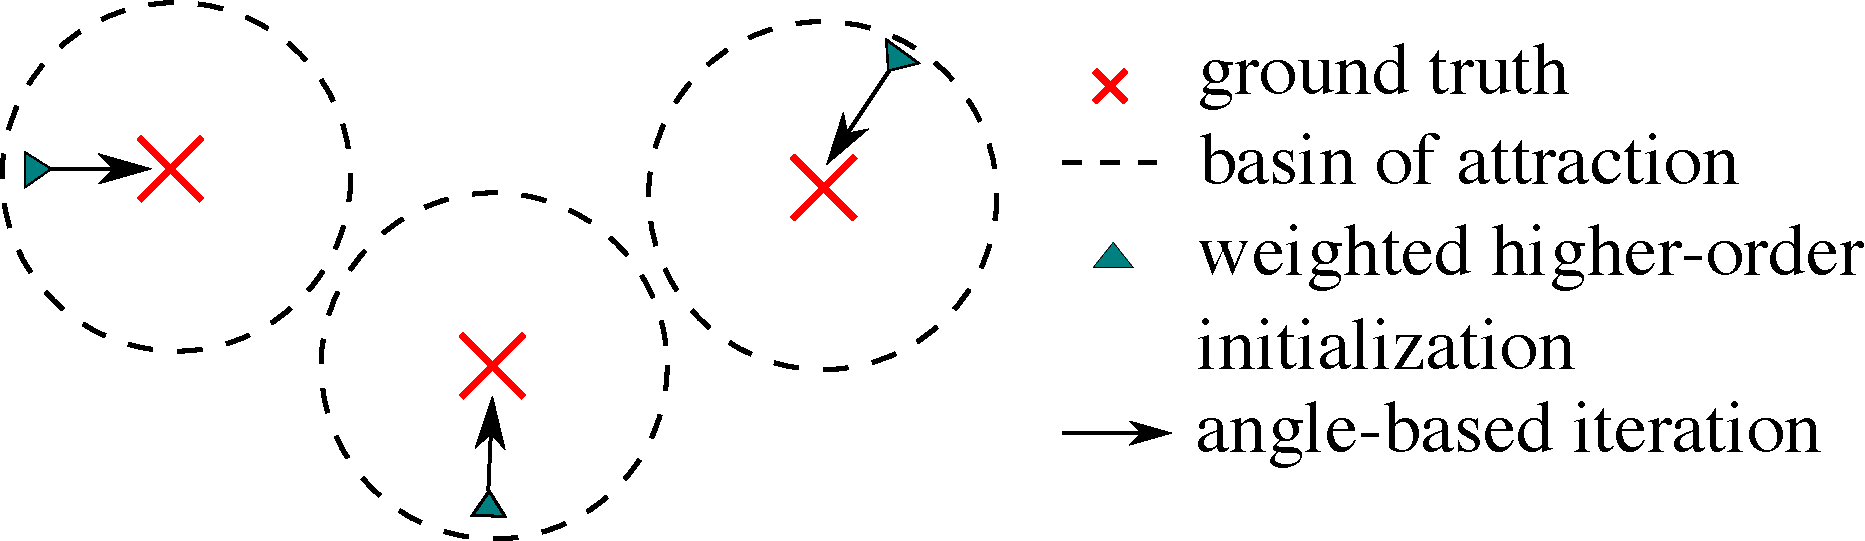
\includegraphics[width=.48\textwidth]{alg_demo.pdf}
%DIFDELCMD < %%%
\DIFdelendFL %DIF > We use the symmetric tensor with i.i.d.\ sub-Gaussian noise to describe the algorithm and develop the theoretical guarantees. 
\DIFaddbeginFL 

\begin{figure}[ht!]
\centering
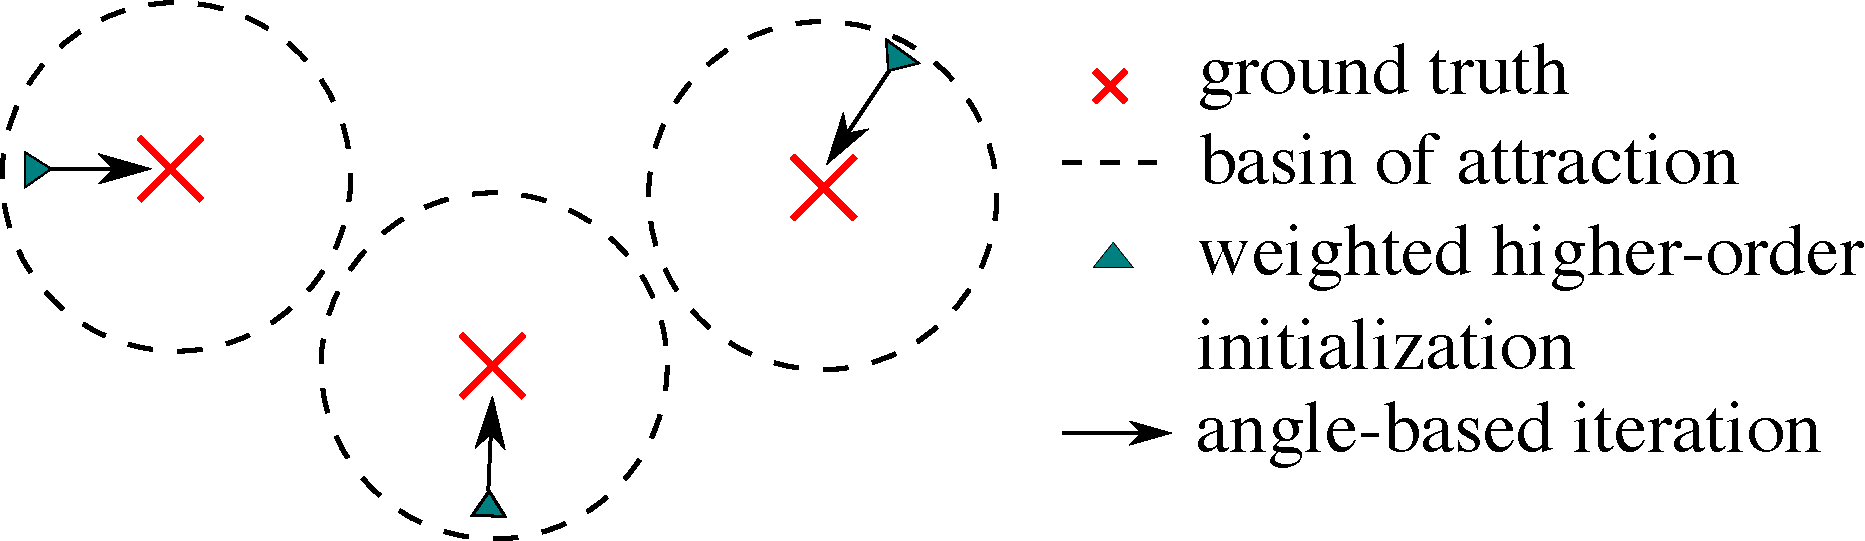
\includegraphics[width=.8\columnwidth]{alg_demo.pdf}
\DIFaddendFL \caption{ \DIFaddbeginFL \small \DIFaddendFL Illustration of our global-to-local algorithm.}\label{fig:demo}
\end{figure}

\DIFdelbegin \subsection{\DIFdel{Weighted higher-order initialization}}
%DIFAUXCMD
\addtocounter{subsection}{-1}%DIFAUXCMD
\DIFdelend \DIFaddbegin \vspace{-.3cm}
\DIFaddend 

\DIFaddbegin \subsection{\DIFadd{Initialization}}

\DIFaddend We start with weighted higher-order clustering algorithm as initialization. \DIFdelbegin \DIFdel{To gain insights, we use }\DIFdelend \DIFaddbegin \DIFadd{We take }\DIFaddend an order-3 symmetric tensor as \DIFdelbegin \DIFdel{a working example}\DIFdelend \DIFaddbegin \DIFadd{illustration for insight}\DIFaddend . Consider noiseless case with $\tX = \bbE\tY$ and $\mX = \text{Mat}(\tX)$. 
By model~\eqref{eq:model_tensor}, for all $i \in [p]$, we have
\begin{equation}\label{eq:kmeans}
    \theta(i)^{-1} \mX_{i:} = \off{\text{Mat}( \tS \times_2 \mTheta \mM \times_3  \mTheta \mM )}_{z(i):}. 
\end{equation}
This implies that, all node $i$ belonging to $a$-th community (i.e., $z(i)=a$) share the same normalized mean vector $\theta(i)^{-1} \mX_{i:}$, and vice versa. Intuitively, one can apply $k$-means clustering to the vectors $\{ \theta(i)^{-1} \mX_{i:} \}_{i\in[p]}$, which leads to main idea of our Sub-algorithm~\hyperref[alg:main]{1}. \DIFdelbegin %DIFDELCMD < 

%DIFDELCMD < %%%
\DIFdelend Specifically, our initialization consists of denoising step and clustering step. The denoising step (lines 1-2 in Sub-algorithm~\hyperref[alg:main]{1}) estimates $\tX$ from $\tY$ by a double projection spectral method.  
%DIF >  The first projection performs HOSVD~\citep{de2000multilinear} via $\mU_{\text{pre}} = \text{SVD}_{r} \of{ \text{Mat}(\tY) }$, where $\text{SVD}_r(\cdot)$ returns the top-$r$ left singular vectors. The second projection performs HOSVD on the projected $\tY$ onto the multilinear Kronecker space $\mU_{\text{pre}} \otimes  \mU_{\text{pre}}$; i.e.,
%DIF >  \begin{equation}\label{eq:two-step_factor}
%DIF >      \hat \mU = \text{SVD}_{r} \of{\text{Mat}\of{ \tY\times_1  \mU_{\text{pre}} \mU_{\text{pre}}^T \times_2   \mU_{\text{pre}} \mU_{\text{pre}}^T }}.
%DIF >  \end{equation}
%DIF >  The final denoised tensor $\hat \tX$ is defined by
%DIF >  \begin{equation}\label{eq:two-step_est}
%DIF >      \hat \tX = \tY \times_1 \hat \mU \hat 
%DIF >  \mU^T \times_2 \hat \mU \hat \mU^T \times_3 \hat \mU \hat \mU^T. 
%DIF >  \end{equation}
The double projection improves usual matrix spectral methods in order to alleviate the noise \DIFdelbegin \DIFdel{tensor.
%DIF < The first projection performs HOSVD~\cite{de2000multilinear} via $\mU_{\text{pre}} = \text{SVD}_{r} \of{ \text{Mat}(\tY) }$, where $\text{SVD}_r(\cdot)$ returns the top-$r$ left singular vectors. The second projection performs HOSVD on the projected $\tY$ onto the multlilinear Kronecker space $\mU_{\text{pre}} \otimes  \mU_{\text{pre}}$; i.e.,
%DIF < \begin{equation}\label{eq:two-step_factor}
 %DIF <    \hat \mU = \text{SVD}_{r} \of{\text{Mat}\of{ \tY\times_1  \mU_{\text{pre}}^T \times_2  \mU_{\text{pre}}^T }}.
%DIF < \end{equation}
%DIF < The final denoised tensor $\hat \tX$ is defined by
%DIF < \begin{equation}\label{eq:two-step_est}
 %DIF <    \hat \tX = \tY \times_1 \hat \mU \hat 
%DIF < \mU^T \times_2 \hat \mU \hat \mU^T \times_3 \hat \mU \hat \mU^T. 
%DIF < \end{equation}
%DIF < Compared with conventional HOSVD, our double projection spectral method is shown to improve the estimation substantially for higher-order tensors~\citep{han2020exact}. 
}\DIFdelend \DIFaddbegin \DIFadd{effects for $K\geq 3$~\mbox{%DIFAUXCMD
\citep{han2020exact}}\hspace{0pt}%DIFAUXCMD
.
}\DIFaddend The clustering step (lines 3-5 in Sub-algorithm~\hyperref[alg:main]{1}) performs the weighted $k$-means clustering. 
%DIF < We write $\hat \mX=\text{Mat}(\hat \tX)$, and normalize the rows into $\hat \mX^s_{i:}=\onormSize{}{\hat \mX_{i:}}^{-1}\hat \mX_{i:}$ as a surrogate of $\theta(i)^{-1} \mX_{i:}$. Then, a weighted $k$-means clustering is performed on the normalized rows with weights equal to $\onormSize{}{\hat \mX_{i:}}^2$. 
%DIF >  We write $\hat \mX=\text{Mat}(\hat \tX)$, and normalize the rows into $\hat \mX^s_{i:}=\onormSize{}{\hat \mX_{i:}}^{-1}\hat \mX_{i:}$ as a surrogate of $\theta(i)^{-1} \mX_{i:}$. Then, a weighted $k$-means clustering is performed on the normalized rows with weights equal to $\onormSize{}{\hat \mX_{i:}}^2$. 
The choice of weights is to bound the $k$-means objective function by the Frobenius-norm accuracy of $\hat \tX$. Unlike existing clustering algorithm~\DIFdelbegin \DIFdel{\mbox{%DIFAUXCMD
\cite{ke2019community}}\hspace{0pt}%DIFAUXCMD
}\DIFdelend \DIFaddbegin \DIFadd{\mbox{%DIFAUXCMD
\citep{ke2019community}}\hspace{0pt}%DIFAUXCMD
}\DIFaddend , we apply the clustering on the unfolded tensor $\hat \mX$ rather than on the factors $\hat \mU$. This strategy relaxes the \DIFdelbegin \DIFdel{eigen-gap separation condition~\mbox{%DIFAUXCMD
\cite{gao2018community, han2020exact}}\hspace{0pt}%DIFAUXCMD
.
%DIF < We assign degenerate rows with purely zero entries to an arbitrarily random cluster; these nodes are negligible in high-dimensions because of the lower bound on $\onormSize{}{\text{Mat}(\tS)_{a:}}$ in~\eqref{eq:family}. The final result gives the initial clustering assignment $\hat z^{(0)}$. 
}\DIFdelend \DIFaddbegin \DIFadd{singular-value gap condition~\mbox{%DIFAUXCMD
\citep{gao2018community, han2020exact}}\hspace{0pt}%DIFAUXCMD
.
%DIF >  We assign degenerate rows with purely zero entries to an arbitrarily random cluster; these nodes are negligible in high-dimensions because of the lower bound on $\onormSize{}{\text{Mat}(\tS)_{a:}}$ in~\eqref{eq:family}. The final result gives the initial cluster assignment $\hat z^{(0)}$.
}\DIFaddend Full procedures are provided in Sub-algorithm~\hyperref[alg:main]{1}. 

\DIFaddbegin \begin{figure*}[h]
    \centering
    \vspace{-.5cm}
    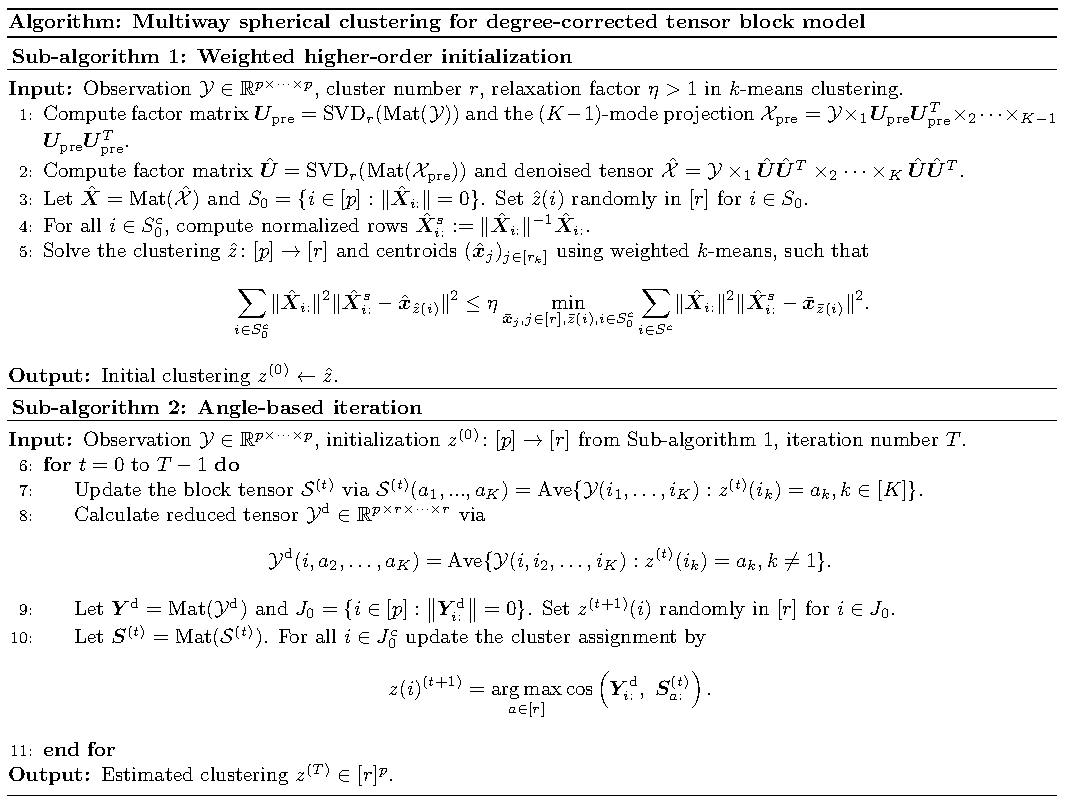
\includegraphics[width=1\textwidth]{algorithm.pdf}
  \vspace{-1cm}
    \label{alg:main}
\end{figure*}


%DIF >  \begin{algorithm}[h!]
%DIF >  \caption*{\bf Algorithm: Multiway spherical clustering for degree-corrected tensor block model }
%DIF >  \vspace{.15cm}
%DIF >  \begin{algorithmic}[1]
%DIF >  \Algphase{Sub-algorithm 1: Weighted higher-order initialization}
%DIF >  \INPUT Observation $\tY \in \bbR^{p\times \cdots \times p}$, cluster number $r$, relaxation factor $\eta > 1$ in $k$-means clustering.
%DIF >  \State Compute factor matrix $ \mU_{\text{pre}} = \text{SVD}_{r} (\text{Mat}(\tY))$ and the $(K-1)$-mode projection $
%DIF >  \tX_{\text{pre}} = \tY \times_1   \mU_{\text{pre}} \mU_{\text{pre}}^T \times_2 \cdots \times_{K-1}  \mU_{\text{pre}} \mU_{\text{pre}}^T.$
%DIF >  \State Compute factor matrix $\hat \mU = \text{SVD}_{r}(\text{Mat}(\tX_{\text{pre}}))$ and denoised tensor
%DIF >  $\hat \tX = \tY \times_1 \hat \mU \hat \mU^T \times_2 \cdots \times_K \hat \mU \hat \mU^T.$
%DIF >  \State {Let $\hat \mX = \text{Mat}(\hat \tX)$ and $S_0=\{i \in [p]: \onormSize{}{\hat \mX_{i:}} = 0\}$. Set $\hat z(i)$ randomly in $[r]$ for $i \in S_0$.}
%DIF >  \State{For all $i\in S_0^c$, compute normalized rows
%DIF >  $\hat \mX_{i:}^s :=\onormSize{}{\hat \mX_{i:}}^{-1} \hat \mX_{i:}.$
%DIF >  }
%DIF >  \State {Solve the clustering $\hat z\colon [p]\to[r]$ and centroids $ (\hat \mx_j)_{j\in[r_k]}$ using weighted $k$-means, such that}
%DIF >  \begin{align}
%DIF >      &\sum_{i \in S_0^c }  \onormSize{}{\hat \mX_{i:}}^2 \onormSize{}{\hat \mX_{i:}^s - \hat \mx_{\hat z(i)} }^2 
%DIF >      \leq 
%DIF >      \eta \min_{\substack{\bar \mx_j, j\in[r], \bar z(i),i\in S_0^{c}}} \sum_{i \in S^c } \onormSize{}{\hat \mX_{i:}}^2 \onormSize{}{ \hat \mX_{i:}^s -   \bar \mx_{\bar z(i)}}^2.
%DIF >  \end{align}
%DIF >  \OUTPUT Initial clustering $z^{(0)} \leftarrow \hat z$.

%DIF >  \Algphase{Sub-algorithm 2: Angle-based iteration}
%DIF >  \INPUT Observation $\tY \in \bbR^{p \times \cdots \times p}$, initialization $z^{(0)} \colon [p]\to[r]$ from Sub-algorithm 1, iteration number $T$.
%DIF >  \For {$t = 0$ to $T-1$}
%DIF >  \State Update the block tensor $\tS^{(t)}$ via
%DIF >  $\tS^{(t)} (a_1,...,a_K)= \text{Ave} \{\tY(i_1,\ldots,i_K): z^{(t)}(i_k) = a_k, k \in [K]\}.$
%DIF >  \State Calculate reduced tensor $\tY^{\text{d}} \in \bbR^{p \times r \times \cdots \times r}$ via
%DIF >  \begin{align}
%DIF >      &\tY^{\text{d}}(i,a_2,\ldots,a_K) 
%DIF >      = 
%DIF >  \text{Ave}\{\tY(i,i_2,\ldots,i_K): z^{(t)}(i_k) = a_k, k \neq 1 \}.
%DIF >  \end{align}

%DIF >  \State Let $\mY^{\text{d}} = \text{Mat}(\tY^{\text{d}})$ and $J_0 = \{ i\in[p]: \onorm{\mY^{\text{d}}_{i:}} = 0\}$. Set $z^{(t+1)}(i)$ randomly in $[r]$ for $i \in J_0$.

%DIF >  \State Let $\mS^{(t)} = \text{Mat}(\tS^{(t)})$. For all $i \in J_0^c$ update the cluster assignment by
%DIF >  \begin{equation}
%DIF >      z(i)^{(t+1)} = \argmax_{a \in [r]} \cos \left( \mY^{\text{d}}_{i:},\ \mS^{(t)}_{a:} \right).
%DIF >  \end{equation}

%DIF >  \EndFor

%DIF >  \OUTPUT Estimated clustering $z^{(T)}  \in [r]^{p}$.

%DIF >  \end{algorithmic}
%DIF >  \end{algorithm}

\DIFaddend We now establish the misclustering error rate of initialization. We call $\mtheta$ is balanced \DIFdelbegin \DIFdel{, }\DIFdelend if the relative extent of heterogeneity is comparable across clusters
\DIFdelbegin \DIFdel{in that
}\DIFdelend \begin{equation}\label{eq:degree}
{\min_{a\in[r]} \onormSize{}{\mtheta_{z^{-1}(a)}}=\left(1+o(1)\right)\max_{a\in[r]}\onormSize{}{\mtheta_{z^{-1}(a)}}}.
\end{equation}
Note that, the assumption~\eqref{eq:degree} does not preclude degree heterogeneity. Indeed, within each of the clusters, the highest degree can be $\theta(i) = \Omega(p)$, whereas the lowest degree can be $\theta(i)=\tO(1)$. 
%DIF < instead, we assume the relative extent of heterogeneity is comparable across clusters.

\DIFdelbegin %DIFDELCMD < \begin{figure*}[h]
%DIFDELCMD <     \centering
%DIFDELCMD <     \vspace{-.5cm}
%DIFDELCMD <     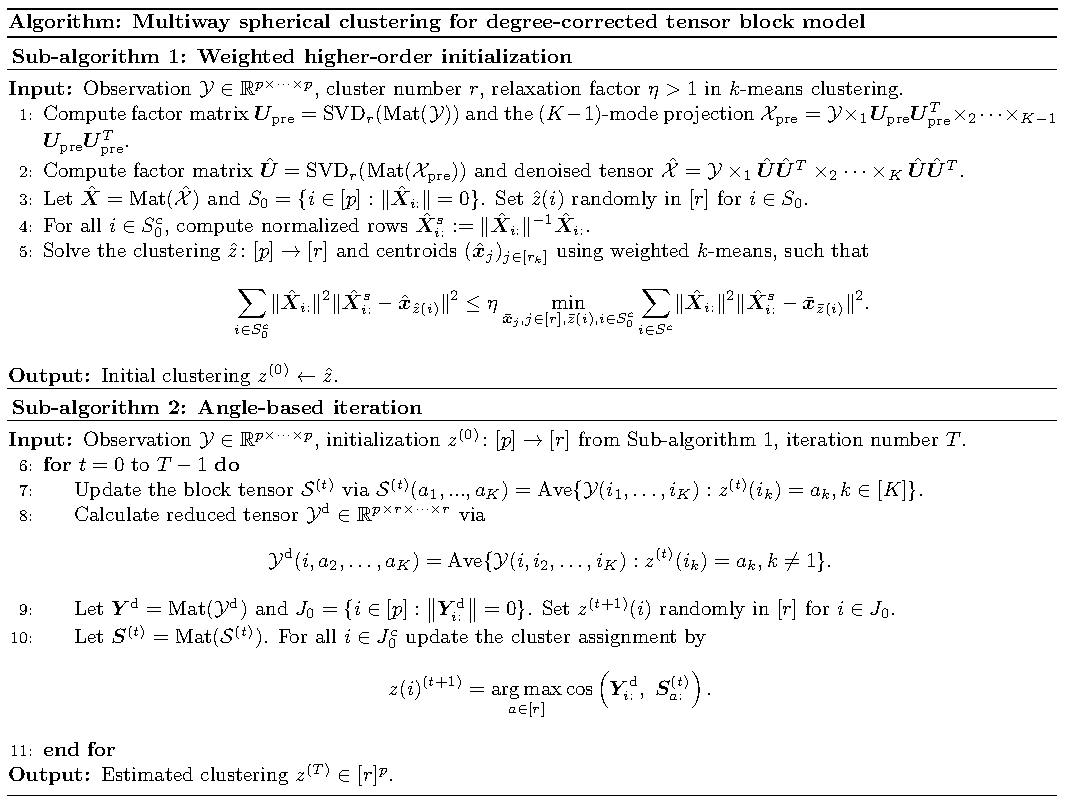
\includegraphics[width=1\textwidth]{algorithm.pdf}
%DIFDELCMD <   \vspace{-1cm}
%DIFDELCMD <     \label{alg:main}
%DIFDELCMD <     %%%
%DIF < \caption{\color{red}\fixme{Jiaxin}{Should be $\argmax_{a \in [r] } \cos \of{ \mY_{i:}^d , \mS_{a:}^{(t)}}$. $\sin$ can not handle the obtuse angles; e.g.\ $\sin \pi = \sin 0= 0$, where $\pi$ is not the desired angle.} \fixme{Miaoyan}{Agree. I corrected it.}}
%DIFDELCMD < \end{figure*}
%DIFDELCMD < 

%DIFDELCMD < %%%
\DIFdelend \begin{thm}[Error for weighted higher-order initialization]\label{thm:initial} Consider the general \DIFdelbegin \DIFdel{Gaussian dTBM }\DIFdelend \DIFaddbegin \DIFadd{sub-Gaussian dTBM with i.i.d.\ noise }\DIFaddend under the parameter space $\tP$ and Assumption~\ref{assmp:min_gap}. %DIF < With probability at least $1 -C \exp(-cp)$, we have
%DIF < \begin{equation}
%DIF < \min_{\pi \in \Pi}\sum_{i\in[p]}\theta^2_i\ind\{ z^{(0)}(i)\neq \pi \circ z(j)\} \lesssim {Mr^K\sigma^2\over \Delta^2_{\min}}p^{-{(K-2)/2}},
%DIF < \end{equation}
%DIF < where $M>1$ is the relation constant in weighted angle $k$-means. 
Assume $\mtheta$ is balanced and $\min_{i\in[p]}\theta(i) \geq c$ for some constant $c>0$. Let $ z^{(0)}$ denote the output of Sub-algorithm~\hyperref[alg:main]{1}. With probability going to 1, we have
\begin{equation}\label{eq:ini}
   \ell(z^{(0)}, z) \lesssim {r^K p^{-K/2} \DIFdelbegin %DIFDELCMD < \over %%%
\DIFdelend \DIFaddbegin \DIFadd{/ }\DIFaddend \text{SNR}}. 
\end{equation}
\end{thm}

\DIFaddbegin \vspace{-.3cm}
\DIFaddend \begin{rmk}[Comparison to previous results] For fixed SNR, our initialization error rate with $K=2$ agrees with the initialization error rate \DIFdelbegin \DIFdel{$\tO(p)$ }\DIFdelend \DIFaddbegin \DIFadd{$\tO(p^{-1})$ }\DIFaddend in matrix models~\DIFdelbegin \DIFdel{\mbox{%DIFAUXCMD
\cite{gao2018community}}\hspace{0pt}%DIFAUXCMD
}\DIFdelend \DIFaddbegin \DIFadd{\mbox{%DIFAUXCMD
\citep{gao2018community}}\hspace{0pt}%DIFAUXCMD
}\DIFaddend . Furthermore, in the special case of non-degree TBMs \DIFaddbegin \DIFadd{with $\theta_1=\cdots=\theta_p=1$}\DIFaddend , we achieve the same initial \DIFdelbegin \DIFdel{misclassification }\DIFdelend \DIFaddbegin \DIFadd{misclustering }\DIFaddend error $\tO(p^{-K/2})$ as in non-degree models~\citep{han2020exact}. Theorem~\ref{thm:initial} implies the advantage of our algorithm in achieving both accuracy and model flexibility. 
%DIF < The result demonstrates the advantage of our algorithm in achieving both accuracy and model flexibility. 
\end{rmk}

%DIF < Assume the number of clusters $r$ is fixed. To ensure the misclassification error $\text{MisClust}(z^{(0)},z)$ decays to 0 as the number of nodes $p \rightarrow \infty$, we need the signal level $\Delta_{\min}^2$ satisfying
%DIF < \begin{equation}
%DIF <     \Delta_{\min}^2/\sigma^2  \gtrsim p^{-K/2}.
%DIF < \end{equation}
%DIF < This implies that desired polynomial rate can be achieved with lower signal level as sample size increases. Moreover, to achieve exact clustering, we should ensure $\text{MisClust}(z^{(0)},z) < \frac{1}{p}$ and thus it requires $\Delta_{\min}^2 \gtrsim p^{2 - K/2}$, which is a fairly strong signal condition especially when $K$ is small. However, the following theorem indicates a weaker signal condition is enough to achieve exact clustering with proper refinement.
\DIFaddbegin \thispagestyle{empty}

\DIFaddend \begin{rmk}[Failure of conventional tensor HOSVD] If we use conventional HOSVD for tensor denoising; that is, we use $\mU_{\text{pre}}$ in place of $\hat \mU$ in line 2, then the misclustering rate becomes \DIFdelbegin \DIFdel{$\tO(p)$ }\DIFdelend \DIFaddbegin \DIFadd{$\tO(p^{-1})$ }\DIFaddend for all $K\geq 2$. This rate is substantially worse than our \DIFdelbegin \DIFdel{current }\DIFdelend rate~\eqref{eq:ini}.
\end{rmk}


\DIFdelbegin %DIFDELCMD < \vspace{-.2cm}
%DIFDELCMD < %%%
\DIFdelend %DIF >  \begin{rmk}[Singular-value gap-free clustering] Note that our clustering directly applies to the estimated mean tensor $\hat \tX$ rather than the leading tensor factors $\hat \mU$. Applying clustering to the tensor factors suffers from the non-identifiability issue due to the infinitely many orthogonal rotations when the number of blocks $r \geq 3$ in the absence of singular-value gaps. 
%DIF >  Such ambiguity causes the trouble for effective clustering~\citep{abbe2020entrywise}. In contrast, our initialization algorithm applies the clustering to the overall mean tensor $\hat \tX$. This strategy avoids the non-identifiability issue regardless of the number of blocks and singular-value gaps.  
%DIF >  \end{rmk}
\DIFaddbegin 


\DIFaddend \subsection{Angle-based \DIFdelbegin \DIFdel{iteration}\DIFdelend \DIFaddbegin \DIFadd{Iteration}\DIFaddend }
%DIF < A polynomial-time local iteration refines the initial spectral clustering to achieve an exponential error rate in TBM~\citep{han2020exact}.  
\DIFaddbegin \DIFadd{Our Theorem~\ref{thm:initial} has shown the polynomially decaying error rate from our initialization. Now we improve the error rate to exponential decay using local iterations. }\DIFaddend We propose an angle-based local iteration to improve the outputs from Sub-algorithm~\hyperref[alg:main]{1}. 
To gain the intuition, consider an one-dimensional degree-corrected clustering problem with data vectors $\mx_i = \theta(i) \ms_{z(i)} + \mepsilon_i, i \in [p]$, where $\ms_i$'s are known cluster centroids, $\theta(i)$'s are unknown \DIFaddbegin \DIFadd{positive }\DIFaddend degrees, and $z\colon [p] \mapsto [r]$ is the \DIFdelbegin \DIFdel{clustering }\DIFdelend \DIFaddbegin \DIFadd{cluster }\DIFaddend assignment of interest. The angle-based $k$-means algorithm estimates the assignment $z$ by minimizing the angle between data vectors and centroids; i.e., 
 \begin{equation}\label{eq:angle_kmeans}
     z(i) = \argmax_{a \in [r]} \cos ( \mx_i,\ \ms_{a} ),\ \text{ for all }i \in [p].
 \end{equation}
\DIFdelbegin \DIFdel{The classical }\DIFdelend \DIFaddbegin \DIFadd{Classical }\DIFaddend Euclidean-distance based clustering~\citep{han2020exact} fails to recover $z$ in the presence of degree heterogeneity, even under noiseless case. In contrast, the \DIFdelbegin \DIFdel{proposed }\DIFdelend angle-based $k$-means achieves accurate recovery without explicit estimation of $\mtheta$.   Our Sub-algorithm~\hyperref[alg:main]{2} shares the same spirit as angle-based $k$-means, except that we use estimated centroids $\ms^{(t)}_a$ in place of $\ms_a$ based on estimated assignment in previous iterations. 
%DIF <  Algorithm~\ref{alg:refinement} updates estimated core tensor and cluster assignments are updated in each iteration. For core tensor, we consider the following update strategy  
 %DIF < \[
%DIF < \tilde \tS(a_1,a_2,a_3)=\text{Ave}\{\tY(i_1,i_2,i_3)\colon z(i_k)=a_k, k\in[3]\}.
%DIF < \]
%DIF < Intuitively, $\tS^{(t)}$ becomes closer to the true core $\tS$ as $z^{(t)}$ is more precise.  we first aggregate the slices of $\tY$ and obtain a reduced tensor $\tY^{\text{d}}\in \bbR^{p \times r \times r}$ with given $z^{(t)}$, where
%DIF < \[
%DIF < \tY^{\text{d}}(i,a_2,a_3)=\text{Ave}\{\tY(i,i_2,i_3)\colon z^{(t)}(i_k)=a_k, k \neq 1\}.
%DIF < \]
%DIF < The row $\text{Mat}(\tY^{\text{d}})_{i:}$ and $\text{Mat}(\tS^{(t)})_{a:}$ corresponds to the $\mx_i$ and $\ms_a$s in the one-dimensional clustering~\eqref{eq:angle_kmeans}. Then, we obtain the updated assignment as
%DIF < \[z(i)^{(t+1)} = \argmin_{a \in [r]} \sin \of{ \mY^{\text{d}}_{i:}, \mS^{(t)}_{a:} }, \text{ for all } i \in [p], \]
%DIF < where $z^{(t+1)}(i)$ is randomly assigned for degenerate rows. 
\DIFdelbegin \DIFdel{Full procedures for our angle-based iteration are described in }\DIFdelend %DIF >  Our Sub-algorithm~\hyperref[alg:main]{2} shares the same spirit as in angle-based $k$-means. We still take the order-3 tensor for illustration. Specifically, Sub-algorithm~\hyperref[alg:main]{2} updates estimated core tensor and cluster assignment in each iteration. We use superscript $\cdot^{(t)}$ to denote the estimate from $t$-th iteration, where $t=1,\ldots.$ For core tensor, we consider the following update strategy 
%DIF >  \small
%DIF >  \begin{equation}
%DIF >       \tS^{(t)}(a_1,a_2,a_3)=\text{Ave}\{\tY(i_1,i_2,i_3)\colon z^{(t)}(i_k)=a_k, k\in[3]\}.
%DIF >  \end{equation}
%DIF >  \normalsize
%DIF >  Intuitively, $\tS^{(t)}$ becomes closer to the true core $\tS$ as $z^{(t)}$ is more precise. For cluster assignment, we first aggregate the slices of $\tY$ and obtain a reduced tensor $\tY^{\text{d}}\in \bbR^{p \times r \times r}$ with given $z^{(t)}$, where
%DIF >  \[
%DIF >  \tY^{\text{d}}(i,a_2,a_3)=\text{Ave}\{\tY(i,i_2,i_3)\colon z^{(t)}(i_k)=a_k, k \neq 1\}.
%DIF >  \]
%DIF >  We use $\mY^d$ and $ \mS^{(t)}$ to denote the $\text{Mat}(\tY^{\text{d}})$ and $\text{Mat}(\tS^{(t)})$. The rows $\mY^d_{i:}$ and $\mS^{(t)}_{a:}$ correspond to the $\mx_i$ and $\ms_a$ in the one-dimensional clustering~\eqref{eq:angle_kmeans}. Then, we obtain the updated assignment by
%DIF >  \[
%DIF >  z(i)^{(t+1)} = \argmax_{a \in [r]} \cos \of{ \mY^{\text{d}}_{i:}, \mS^{(t)}_{a:} },\ \text{ for all } i \in [p],
%DIF >  \]
%DIF >  provided that $\mS^{(t)}_{a:}$ is a non-zero vector. Otherwise, if $\mS^{(t)}_{a:}$ is a zero vector, then we make the convention to assign $z^{(t+1)}(i)$ randomly in $[p]$. 
\DIFaddbegin \DIFadd{See }\DIFaddend Sub-algorithm~\hyperref[alg:main]{2} \DIFdelbegin \DIFdel{. The following theorem establishes }\DIFdelend \DIFaddbegin \DIFadd{for full procedures.
}

\DIFadd{We now establish }\DIFaddend the misclustering error rate of iterations \DIFaddbegin \DIFadd{under the stability assumption}\DIFaddend .

%DIF <   In Algorithm~\ref{alg:refinement}, the estimated core tensor and cluster assignments are updated in each iteration. For core tensor, notice that the estimator $\tilde S$ with
%DIF <    \[
%DIF <  \tilde \tS(a_1,a_2,a_3)=\text{Ave}\{\tY(i_1,i_2,i_3)\colon z(i_k)=a_k, k\in[3]\}
%DIF <  \]
%DIF <  is an unbiased estimator satisfying $\bbE[\tilde \tS_{a_1,...,a_K}] = \tS_{a_1,...,a_K}$ with true assignment $z$. This leads to a reasonable core tensor update strategy 
%DIF <   \[
%DIF <  \tS^{(t)}(a_1,a_2,a_3)=\text{Ave}\{\tY(i_1,i_2,i_3)\colon z^{(t)}(i_k)=a_k, k\in[3]\}.
%DIF <  \]
%DIF <  Intuitively, the estimate $\tS^{(t)}$ becomes better as $z^{(t)}$ getting more precise. 
\DIFaddbegin \thispagestyle{empty}
\DIFaddend 

%DIF <  For cluster assignment, we reduce the higher-order problem to the one-dimensional clustering by matrization. Given $z^{(t)}$, we first aggregate the slices of $\tY$ and obtain a reduced tensor $\tY^{\text{d}}\in \bbR^{p \times r \times r}$, where
%DIF <  \[
%DIF <  \tY^{\text{d}}(i,a_2,a_3)=\text{Ave}\{\tY(i,i_2,i_3)\colon z^{(t)}(i_k)=a_k, k \neq 1\}.
%DIF <  \]
%DIF <  Let $\mY^{\text{d}} = \text{Mat}(\tY^{\text{d}})$ and $\mS^{(t)} = \text{Mat}(\tS^{(t)})$. Then, the row $\mY^{\text{d}}_{i:}$s and $\mS^{(t)}_{a:}$s serve as the data vectors $\mx_i$ and centroids $\ms_a$s in the one-dimensional clustering~\eqref{eq:angle_kmeans}. We obtain the updated assignment as
%DIF <  \begin{equation}
%DIF <      z(i)^{(t+1)} = \argmin_{a \in [r]} \sin \of{ \mY^{\text{d}}_{i:}, \mS^{(t)}_{a:} }, \text{ for all } i \in [p].
%DIF <  \end{equation}
%DIF <  In particular, $z^{(t+1)}(i)$ is randomly assigned for degenerate row with $\onorm{\mY^{\text{d}}_{i:}} = 0$. The refinement outputs the final cluster assignment after $T$ iterations denoted $z^{(T)}$. The full procedure for general order-$K$ tensor is described in Algorithm~\ref{alg:refinement}
\DIFaddbegin \begin{defn}[Locally linear stability] \label{def:stable}
\DIFadd{Define the $\varepsilon$-neighborhood of $z$ by $\tN(z,\varepsilon)=\{\bar z\colon \ell(\bar z, z) \leq \varepsilon\}$. Let $\bar z\colon[p]\to [r]$ be a clustering function. The degree is $\varepsilon$-locally linearly stable if and only if
}\begin{equation}\DIFadd{\label{eq:local}
    \sin(\mp(\bar z),\ \mp_{\mtheta}(\bar z))\lesssim \varepsilon \Delta_{\min} ,\text{ for all } \bar z\in \tN(z, \varepsilon),
}\end{equation}
\DIFadd{where $\mp(\bar z)=(|\bar z^{-1}(1)|, \ldots,|\bar z^{-1}(r)|)^T$ and $\mp_{\mtheta}(\bar z)=(\onormSize{}{\mtheta_{\bar z^{-1}(1)}}_1,\ldots,\onormSize{}{\mtheta_{\bar z^{-1}(r)}}_1)^T$.
%DIF >  We define two vectors associated with $\bar z$,
%DIF >  \small
%DIF >  \begin{align}
%DIF >      &\mp(\bar z)=(|\bar z^{-1}(1)|, \ldots,|\bar z^{-1}(r)|)^T, \\
%DIF >      &\mp_{\mtheta}(\bar z)=(\onormSize{}{\mtheta_{\bar z^{-1}(1)}}_1,\ldots,\onormSize{}{\mtheta_{\bar z^{-1}(r)}}_1)^T.
%DIF >  \end{align}
%DIF >  \normalsize
}\end{defn}
\DIFadd{Roughly speaking, the vector $\mp(\bar z)$ represents the raw cluster sizes, and $\mp_{\theta}(\bar z)$ represents the relative cluster sizes weighted by degrees. 
The local stability holds trivially for $\varepsilon=0$ based on the construction of parameter space~}\eqref{eq:family}\DIFadd{. The condition~}\eqref{eq:local} \DIFadd{controls the impact of node degree to the $\mp_{\theta}(\cdot)$ with respect to the misclassification rate $\varepsilon$ and angle gap.
 }\DIFaddend 

\begin{thm}[Error for angle-based iteration]\label{thm:refinement} Consider the setup as in Theorem~\ref{thm:initial}. Suppose 
$r=\tO(1)$ and \DIFdelbegin \DIFdel{$\text{SNR} \gtrsim  p^{-K/2}$. }\DIFdelend \DIFaddbegin \DIFadd{$\text{SNR} \geq \tilde C p^{-K/2}\log p$ for some sufficiently large constant $\tilde C$. Assume the local linear stability of degree holds in the neighborhood $\tN(z,\varepsilon)$ for all $\varepsilon \leq E_0$ and some $E_0 \geq \check{C}\log^{-1}p $ with some positive constant $\check{C}$.  }\DIFaddend Let $z^{(t)}$ denote the $t$-th iteration output in Sub-algorithm~\hyperref[alg:main]{2} with initialization $z^{(0)}$ from Sub-algorithm~\hyperref[alg:main]{1}. With probability going to 1, there exists a contraction parameter $\rho \in (0,1)$ such that 
\DIFdelbegin %DIFDELCMD < 

%DIFDELCMD < %%%
\DIFdelend {\footnotesize
\DIFdelbegin %DIFDELCMD < \vspace{-.4cm}
%DIFDELCMD < %%%
\begin{align*}\DIFdel{%DIFDELCMD < \label{eq:final}%%%
    \ell(z, \hat z^{(t+1)}) \lesssim }&\DIFdel{\ \KeepStyleUnderBrace{
   \text{SNR}^{-1}
    \exp\of{- \frac{p^{K-1}\text{SNR}}{r^{K-1}}}}_{\substack{\text{statistical}\\ \text{error}} }+ \KeepStyleUnderBrace{ \rho^t \ell(z, z^{(0)}). }_{\substack{\text{computational}\\ \text{error}}}
}\end{align*}%DIFAUXCMD
\DIFdelend \DIFaddbegin \vspace{-.1cm}
\begin{equation}\DIFadd{\label{eq:final}
     \ell(z, \hat z^{(t+1)}) \lesssim  \ \KeepStyleUnderBrace{
   \text{SNR}^{-1}
    \exp\of{- \frac{p^{K-1}\text{SNR}}{r^{K-1}}}}_{\substack{\text{statistical error}} }+ \KeepStyleUnderBrace{ \rho^t \ell(z, z^{(0)}). }_{\substack{\text{computational}\\ \text{error}}}
}\end{equation}\DIFaddend 
\vspace{-.4cm}
}
\end{thm}
\DIFdelbegin %DIFDELCMD < \normalsize
%DIFDELCMD < %%%
\DIFdelend The iteration error is decomposed into two parts: statistical error and computational error. The statistical error is unavoidable with noisy data regardless $t$, whereas the computational error decays in an exponential rate as the number of iterations $t \rightarrow \infty$. \DIFdelbegin %DIFDELCMD < 

%DIFDELCMD < %%%
\DIFdelend Theorem~\ref{thm:refinement} implies that, with probability going to 1, our estimate $z^{(T)}$ achieves exact recovery within polynomial iterations; more precisely,
\DIFaddbegin \vspace{-.1cm}
\DIFaddend \begin{equation}
     z^{(T)} = \pi \circ z, \quad \text{for all }T\gtrsim \log_{1/\rho} p,
\end{equation}
for some permutation $\pi \in \Pi$. %DIF < We now discuss the conditions for which exact recovery occurs, i.e., $\ell(z, \hat z^{(t+1)})=0$ for some $t\geq T=\text{poly}(p)$. Based on Theorem~\ref{thm:refinement}, we need
%DIF < \[
%DIF < T\geq \log p +\log \ell(z, \hat z^{(0)})
%DIF < \]
%DIF < given initial assignment $z^{(0)}$ from Algorithm~\ref{alg:initial} and iteration number $T \geq 2 \log p$, with probability going to 1, the output of our Algorithm~\ref{alg:refinement} achieves exact recovery, i.e., for some permutation $\pi \in \Pi$,
%DIF < \begin{equation}
 %DIF <     z^{(T)} = \pi \circ z, \quad \text{for all }T\geq 2\log p.
%DIF < \end{equation}
\DIFaddbegin \DIFadd{Hence, our combined algorithm is }\textit{\DIFadd{computationally efficient}} \DIFadd{as long as SNR $\gtrsim p^{-K/2} \log p$. Note that, ignoring the logarithmic term, the minimal SNR requirement, $p^{-K/2}$, coincides with the computational lower bound in Theorem~\ref{thm:comp}. Therefore, our algorithm is optimal regarding the signal requirement and lies in the sharpest }\emph{\DIFadd{computationally efficient}} \DIFadd{regime in Figure~\ref{fig:phase_axis}.
}\DIFaddend 

%DIF < \begin{algorithm}[h]
\DIFaddbegin \thispagestyle{empty}
%DIF > \subsection{Extensions \& Practical Issues}~\label{subsec:exten}
\DIFaddend 

%DIF < \caption{Angle-based iteration}\label{alg:refinement}
%DIF < \begin{algorithmic}[1]
\DIFdelbegin %DIFDELCMD < 

%DIFDELCMD < %%%
%DIF < \INPUT Observation $\tY \in \bbR^{p \times \cdots \times p}$, initialization $z^{(0)} \colon [p]\to[r]$, iteration number $T$.
%DIF < \For {$t = 0$ to $T-1$}
%DIF < \State Update the block tensor $\tS^{(t)}$ via
%DIF < \begin{align}
%DIF <     &\tS^{(t)} (i_1,...,i_K)\\
 %DIF <    & \quad = \text{Ave} \{\tY(i_1,\ldots,i_K): z^{(t)}(i_k) = j_k, k \in [K]\}
%DIF < \end{align}
%DIF < \State Calculate reduced tensor $\tY^{\text{d}} \in \bbR^{p \times r \times \cdots \times r}$
%DIF < \begin{align}
%DIF <     &\tY^{\text{d}}(i,a_2,\ldots,a_%K) \\
%DIF <     &= 
%DIF < \text{Ave}\{\tY(i,i_2,\ldots,i_K): z^{(t)}(i_k) = a_k, k \neq 1 \}
%DIF < \end{align}
%DIFDELCMD < 

%DIFDELCMD < %%%
%DIF < \State Let $\mY^{\text{d}} = \text{Mat}(\tY^{\text{d}})$ and $J_0 = \{ i\in[p]: \onorm{\mY^{\text{d}}_{i:}} = 0\}$. Set $z^{(t+1)}(i)$ randomly in $[r]$ for $i \in J_0$.
%DIFDELCMD < 

%DIFDELCMD < %%%
%DIF < \State Let $\mS^{(t)} = \text{Mat}(\tS^{(t)})$. For all $i \in J_0^c$ update cluster assignment by
%DIF < \begin{equation}
%DIF <     z(i)^{(t+1)} = \argmin_{a \in [r]} \sin \of{ \mY^{\text{d}}_{i:}, \mS^{(t)}_{a:} }.
%DIF < \end{equation}
%DIFDELCMD < 

%DIFDELCMD < %%%
%DIF < \EndFor
%DIFDELCMD < 

%DIFDELCMD < %%%
%DIF < \OUTPUT Estimated clustering $z^{(T)}  \in [r]^{p}$.
%DIF < \end{algorithmic}
%DIF < \end{algorithm}
%DIFDELCMD < 

%DIFDELCMD < %%%
%DIF < We refer to the combination of Algorithms~\ref{alg:initial}+ \ref{alg:refinement} as provable dTBM algorithm. 
%DIFDELCMD < 

%DIFDELCMD < %%%
%DIF < \fixme{Miaoyan}{add discussion as in my JMLR binary tensor paper (stat-comp dominating terms)}
%DIFDELCMD < 

%DIFDELCMD < %%%
\DIFdelend \section{\DIFdelbegin \DIFdel{Numerical studies}\DIFdelend \DIFaddbegin \DIFadd{NUMERICAL STUDIES}\DIFaddend }\label{sec:simulation}

 We evaluate the performance of \DIFdelbegin \DIFdel{the weighted higher-order initialization and angle-based iteration }\DIFdelend \DIFaddbegin \DIFadd{our algorithm }\DIFaddend in this section. We report average errors and standard deviations across 30 replications in each experiment. Clustering accuracy is assessed by clustering error rate (CER, i.e., one minus rand index). Note that CER between $(\hat z, z)$ is equivalent to misclustering error $\ell(\hat z, z)$ up to constant multiplications~\citep{meilua2012local}, and \DIFdelbegin \DIFdel{a }\DIFdelend lower CER indicates \DIFdelbegin \DIFdel{a }\DIFdelend better performance. 

We generate order-3 tensors with \emph{assortative}~\DIFdelbegin \DIFdel{\mbox{%DIFAUXCMD
\cite{gao2018community} }\hspace{0pt}%DIFAUXCMD
}\DIFdelend \DIFaddbegin \DIFadd{\mbox{%DIFAUXCMD
\citep{gao2018community} }\hspace{0pt}%DIFAUXCMD
}\DIFaddend core tensors to control SNR; i.e., we set $\tS_{aaa} = s_1$ for $a \in [r]$ and others be $s_2$, where $s_1 > s_2 > 0$. Let $\alpha = s_1/s_2$. We set $\alpha$ close to 1 such that $1-\alpha=o(p)$. In particular, we have $\alpha = 1 + \Omega(p^{\gamma/2})$ %DIF < \fixme{Miaoyan}{My calculation shows $\text{SNR}=\Omega((1-\alpha)^2)\Rightarrow \alpha=1+\Omega(p^{\gamma/2})$. Double check.} 
  \DIFaddbegin \DIFadd{with $\gamma<0$ }\DIFaddend by Assumption~\ref{assmp:min_gap} and definition~\eqref{eq:gamma}. Hence, we easily adjust SNR via varying $\alpha$. %DIF < We also set $\onorm{\text{Mat}(\tS)_{a:}} = c$ for some $c>0$ to exclude the effect of signal magnitude. 
 \DIFdelbegin \DIFdel{Note that the }\DIFdelend \DIFaddbegin \DIFadd{The }\DIFaddend assortative setting is proposed for simulations, and our algorithm is applicable for general tensors in practice. The cluster assignment $z$ is randomly generated with equal probability across  $r$ clusters for each mode. Without further explanation, we generate degree heterogeneity $\mtheta$ from absolute normal distribution \DIFdelbegin \DIFdel{as }\DIFdelend \DIFaddbegin \DIFadd{by }\DIFaddend $\theta(i) = |X_i| + 1 - 1/\sqrt{2\pi}$ with $|X_i| \stackrel{\text{i.i.d.}}\sim N(0,1), i \in [p]$ and normalize $\mtheta$ to satisfy \eqref{eq:family}. We set $\sigma^2 = 1$ for Gaussian data.

%DIF <   To control SNR, we generate ``assortative" core tensors for all experiments, as a higher-order analogy of the setting in \cite{gao2018community}; i.e.,
%DIF <  \begin{align} \tS_{ijk} = 
%DIF <      \begin{cases}
%DIF <      s_1 & \text{if } i = j = k,\\
%DIF <      s_2 & \text{if $i,j,k$ are not identical, }
%DIF <      \end{cases}
%DIF <  \end{align}
%DIF <  where $s_1 > s_2 > 0$. Let $\alpha = s_1/s_2$ be the ratio between diagonal and off-diagonal elements. We have $\alpha = 1 + \Omega(p^{\gamma})$ by Assumption~\ref{assmp:min_gap} and definition~\eqref{eq:gamma} with fixed $\sigma^2$. This helps us to easily adjust SNR via varying $\alpha$. We also set $\onorm{\text{Mat}(\tS)_{a:}} = c$ for some $c>0$ to exclude the effect of signal magnitude. The ``assortative" setting is proposed for convenience. In practice, our algorithm is applicable for general core tensor. 
\DIFaddbegin \subsection{\DIFadd{Verification of Theoretical Results}}\label{subsec:num_theory}
\DIFaddend 

%DIF <  The cluster assignment $z$ is randomly generated with given integer $r$. Without specific explanation, we generate degree heterogeneity $\mtheta$ from absolute normal distribution as $\theta(i) = |X_i| + 1 - 1/\sqrt{2\pi}, i \in [p]$ with $|X_i| \sim_{i.i.d.} N(0,1)$ and normalize $\mtheta$ to satisfy \eqref{eq:family}. We generate the noisy tensor under Gaussian model with $\sigma^2 = 1$ and Bernoulli model with mean tensor  $\tS \times_1 \mTheta \mM \times_2 \mTheta \mM \times_3 \mTheta \mM$. We denote provable dTBM algorithm as \textbf{Ours} for simplicity.
\DIFaddbegin \begin{figure}[htb]
    \centering
    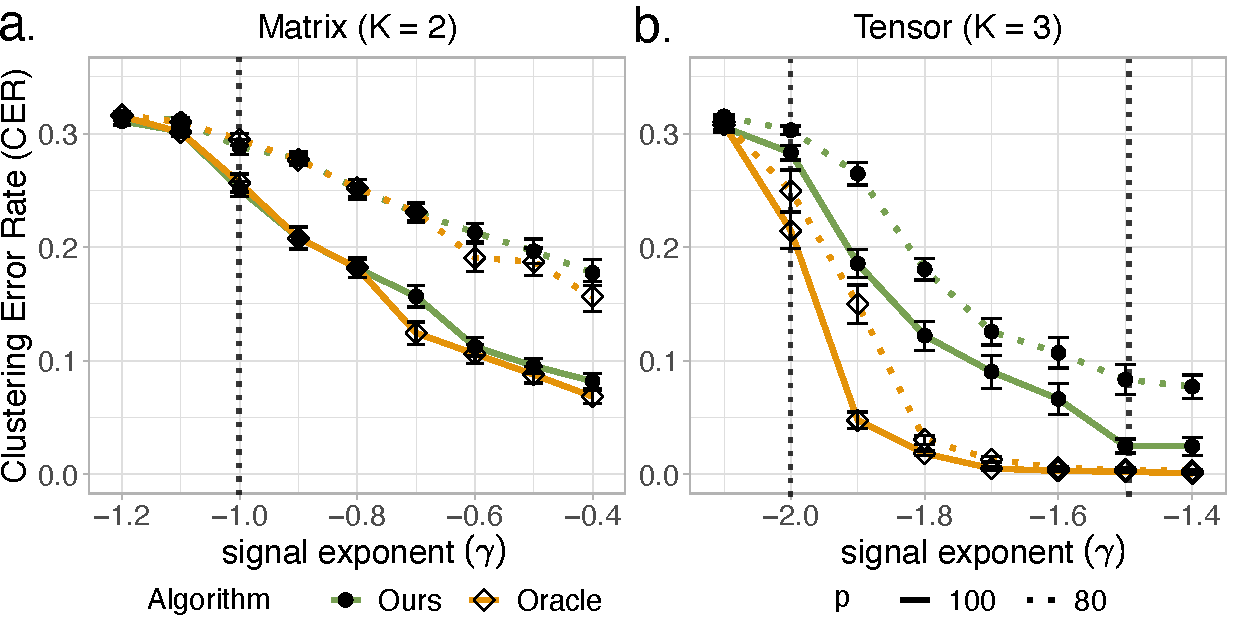
\includegraphics[width=.95\columnwidth]{phase_anno.pdf}
    \caption{ \footnotesize \DIFaddFL{SNR phase transitions for clustering in dTBM with $p = \{80, 100\}, r = 5$ under (a) matrix case with $\gamma \in [-1.2, -0.4]$ and (b) tensor case with $ \gamma \in [-2.1, -1.4]$.
    }}
    \label{fig:phase}
    \vspace{-.5cm}
\end{figure}
\DIFaddend 

\DIFdelbegin \subsection{\DIFdel{Verification for theoretical results}}
%DIFAUXCMD
\addtocounter{subsection}{-1}%DIFAUXCMD
\DIFdelend \DIFaddbegin \begin{figure}[htb]
    \centering
     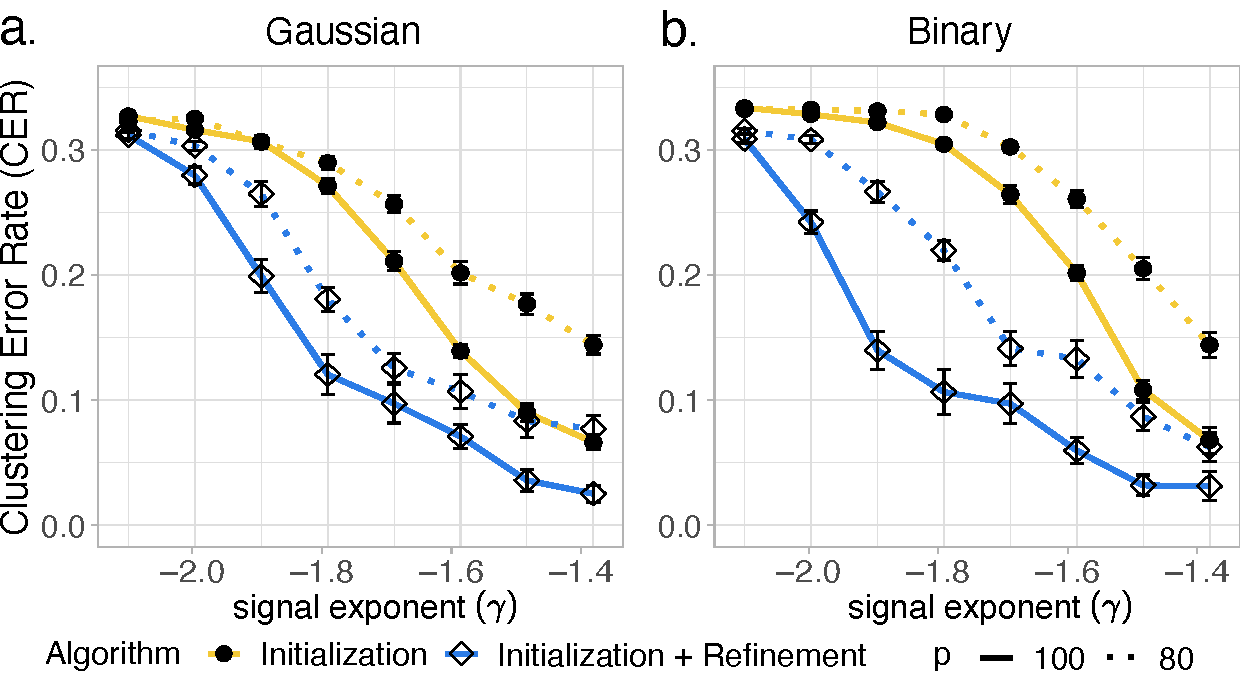
\includegraphics[width=.95\columnwidth]{ini_re_anno.pdf}
    \caption{ \footnotesize \DIFaddFL{CER versus signal exponent $(\gamma)$ for initialization only and for combined algorithm. We set $p = \{80, 100\}, r = 5, \gamma \in [-2.1, -1.4]$ under (a) Gaussian models and (b) Bernoulli models. }}
    \label{fig:ini_re}
    \vspace{-.5cm}
\end{figure}
\DIFaddend 

The first experiment verifies  statistical-computational gap described in Section~\ref{sec:limits}. Consider the Gaussian model with $p = \{80, 100\}$, $r = 5$. We vary $\gamma $ in $ [-1.2, -0.4]$ and $[-2.1, -1.4]$ for matrix ($K=2$) and tensor $(K = 3)$ clustering, respectively. Note that finding MLE under dTBM is computationally intractable. We approximate MLE using an oracle estimator\DIFdelbegin \DIFdel{; }\DIFdelend \DIFaddbegin \DIFadd{, }\DIFaddend i.e., the output of Sub-algorithm~\hyperref[alg:main]{2} initialized from true assignment. \DIFdelbegin \DIFdel{Fig.}\DIFdelend \DIFaddbegin \DIFadd{Figure}\DIFaddend ~\ref{fig:phase}a shows that both our algorithm and oracle estimator start to decrease around the critical value $\gamma_{\text{stat}}  = \gamma_{\text{comp}}  = -1$ in matrix case. In contrast, \DIFdelbegin \DIFdel{Fig.}\DIFdelend \DIFaddbegin \DIFadd{Figure}\DIFaddend ~\ref{fig:phase}b shows a significant gap in the phase transitions between the algorithm estimator and oracle estimator in tensor case. The oracle error rapidly decreases to 0 when $\gamma_{\text{stat}} = -2$, whereas the algorithm estimator tends to achieve exact clustering when $\gamma_{\text{comp}} = -1.5$. \DIFdelbegin \DIFdel{Fig.}\DIFdelend \DIFaddbegin \DIFadd{Figure}\DIFaddend ~\ref{fig:phase} confirms the existence of the statistical-computational gap in our Theorems~\ref{thm:stats} and~\ref{thm:comp}. 

\DIFdelbegin %DIFDELCMD < \begin{figure}[htb]
%DIFDELCMD <     \centering
%DIFDELCMD <     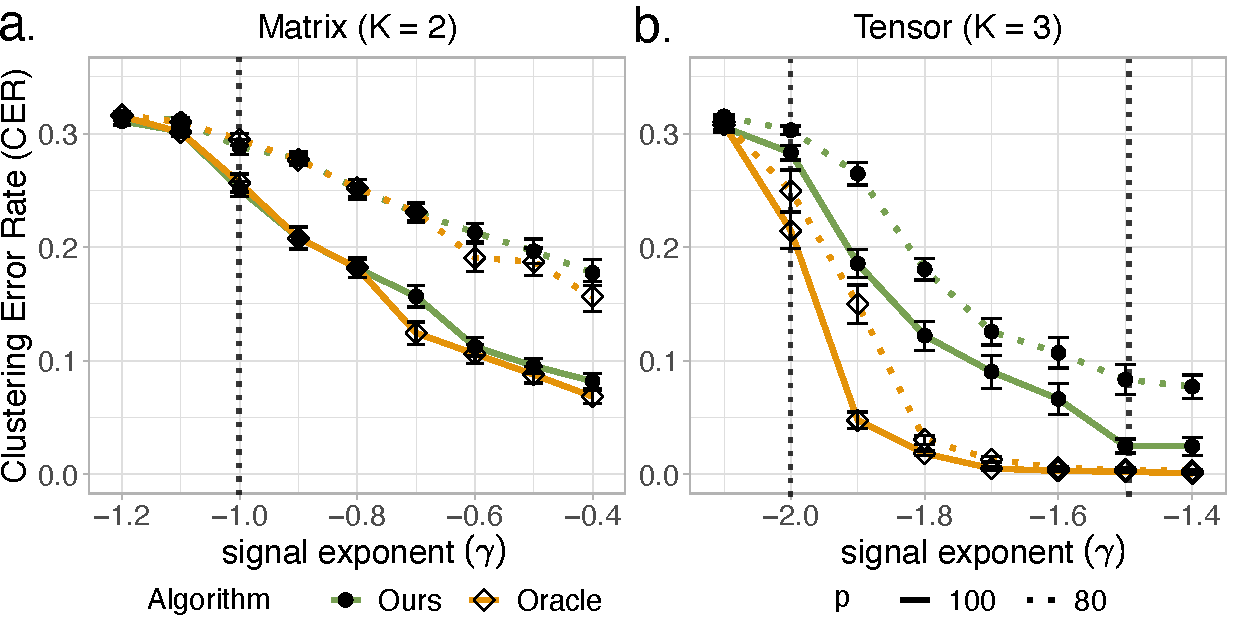
\includegraphics[width=.48\textwidth]{phase_anno.pdf}
%DIFDELCMD <     %%%
%DIFDELCMD < \caption{%
{%DIFAUXCMD
%DIFDELCMD < \footnotesize %%%
\DIFdelFL{SNR phase transitions for clustering in dTBM with $p = \{80, 100\}, r = 5$ under (a) matrix case with $\gamma \in [-1.2, -0.4]$ and (b) tensor case with $ \gamma \in [-2.1, -1.4]$.
    }}
    %DIFAUXCMD
%DIFDELCMD < \label{fig:phase}
%DIFDELCMD < \end{figure}
%DIFDELCMD < 

%DIFDELCMD < %%%
\DIFdelend The second experiment verifies the performance guarantees of two algorithms: (i) weighted higher-order initialization; (ii) combined algorithm of weighted higher-order initialization and angle-based iteration. We consider both the Gaussian and Bernoulli models with $p = \{80, 100\}$, $r = 5$, $\gamma \in [-2.1, -1.4]$. %DIF < We set $c = 0.5$ and $c = 0.25$ for Gaussian and Bernoulli cases, respectively. 
\DIFdelbegin \DIFdel{Fig.}\DIFdelend \DIFaddbegin \DIFadd{Figure}\DIFaddend ~\ref{fig:ini_re} shows the substantial improvement of combined algorithm over initialization, especially under weak and intermediate signals. This phenomenon agrees with the error rates in Theorems~\ref{thm:initial} and \ref{thm:refinement} 
and confirms the necessity of the local iterations.



\DIFdelbegin %DIFDELCMD < \begin{figure}[h!]
%DIFDELCMD <     \centering
%DIFDELCMD <      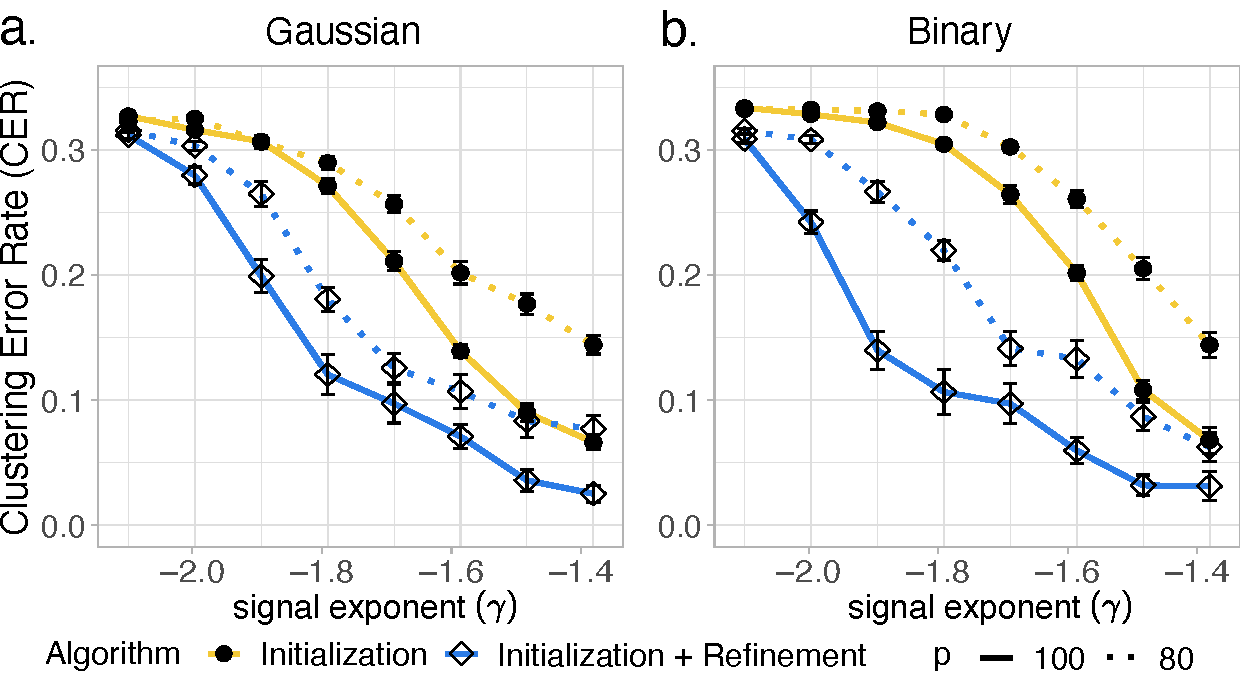
\includegraphics[width=.48\textwidth]{ini_re_anno.pdf}
%DIFDELCMD <     %%%
%DIFDELCMD < \caption{%
{%DIFAUXCMD
%DIFDELCMD < \footnotesize %%%
\DIFdelFL{CER versus signal exponent $(\gamma)$ for initialization only and for combined algorithm. We set $p = \{80, 100\}, r = 5, \gamma \in [-2.1, -1.4]$ under (a) Gaussian models with $c = 0.5$ and (b) Bernoulli models with $c = 0.25$. }}
    %DIFAUXCMD
%DIFDELCMD < \label{fig:ini_re}
%DIFDELCMD <         \vspace{-.2cm}
%DIFDELCMD < \end{figure}
%DIFDELCMD < 

%DIFDELCMD < %%%
\DIFdelend \subsection{Comparison with \DIFdelbegin \DIFdel{other methods}\DIFdelend \DIFaddbegin \DIFadd{Other Methods}\DIFaddend }\label{subsec:comp}
\DIFdelbegin %DIFDELCMD < 

%DIFDELCMD < %%%
\DIFdel{We compare }\DIFdelend \DIFaddbegin \DIFadd{Compare }\DIFaddend our algorithm with \DIFdelbegin \DIFdel{following higher-order clustering methods }\DIFdelend \DIFaddbegin \DIFadd{methods below}\DIFaddend :
\begin{itemize}[wide,topsep=-3pt,itemsep=0pt,parsep=1pt]
    \item \textbf{\small HOSVD}: HOSVD on data tensor and $k$-means on the rows of the factor matrix;
    \item \textbf{\small HOSVD+}: HOSVD on data tensor and $k$-means on the $\ell_2$-normalized rows of the factor matrix;
    \item \textbf{\small HLloyd}\DIFaddbegin \DIFadd{~\mbox{%DIFAUXCMD
\citep{han2020exact}}\hspace{0pt}%DIFAUXCMD
}\DIFaddend : High-order \DIFdelbegin \DIFdel{Lloyd algorithm and high-order spectral clustering ~\mbox{%DIFAUXCMD
\citep{han2020exact}}\hspace{0pt}%DIFAUXCMD
}\DIFdelend \DIFaddbegin \DIFadd{clustering algorithm developed for non-degree TBM}\DIFaddend ;
    \item \textbf{\small SCORE}\DIFaddbegin \DIFadd{~\mbox{%DIFAUXCMD
\citep{ke2019community}}\hspace{0pt}%DIFAUXCMD
}\DIFaddend : Tensor-SCORE for clustering \DIFdelbegin \DIFdel{~\mbox{%DIFAUXCMD
\citep{ke2019community}}\hspace{0pt}%DIFAUXCMD
;
    %DIF < \item \textbf{\small SCORE-}: Incomplete tensor-SCORE without regularized higher-order orthogonal iteration.
}\DIFdelend \DIFaddbegin \DIFadd{developed for binary tensors.
}\DIFaddend \end{itemize}

Among the four alternative algorithms, the \textbf{\small SCORE} is the closest method to ours. %DIF < , since \textbf{\small SCORE} also The incomplete version \textbf{\small SCORE-} skips the key step, regularized HOOI, in \textbf{\small SCORE}. We involve \textbf{\small SCORE-} to study the critical components of \textbf{\small SCORE}. 
We set the tuning parameters of \textbf{\small SCORE} as in previous literature \DIFdelbegin \DIFdel{\mbox{%DIFAUXCMD
\cite{ke2019community}}\hspace{0pt}%DIFAUXCMD
}\DIFdelend \DIFaddbegin \DIFadd{\mbox{%DIFAUXCMD
\citep{ke2019community}}\hspace{0pt}%DIFAUXCMD
}\DIFaddend . The methods \textbf{\small SCORE} and \textbf{\small HOSVD+} are designed for \DIFdelbegin \DIFdel{degree models}\DIFdelend \DIFaddbegin \DIFadd{dTBM~}\eqref{eq:model_tensor}\DIFaddend , whereas \textbf{\small HOSVD} and \textbf{\small HLloyd} are designed for non-degree models \DIFdelbegin \DIFdel{.
%DIF < which shares a similar idea of our spectral initialization but implements naive denoising and clustering steps.  We refer our algorithm as \textbf{\small dTBM}.
%DIF < , and the later one is expected to outperform than spectral methods under TBM. 
}\DIFdelend \DIFaddbegin \DIFadd{serving as benchmarks. }\DIFaddend We conduct two experiments to assess the impacts of (i) signal strength and (ii) degree heterogeneity \DIFdelbegin \DIFdel{, based on }\DIFdelend \DIFaddbegin \DIFadd{under }\DIFaddend Gaussian and Bernoulli models with $ p = 100, r = 5$. We \DIFdelbegin \DIFdel{refer to }\DIFdelend \DIFaddbegin \DIFadd{call }\DIFaddend our algorithm as \textbf{\small dTBM} in the comparison. 
%DIF < Consider $ p = 100, r = 5, c = 0.5$ for both experiments. 

We investigate the effects of signal to clustering performance by varying $\gamma \in [-1.5, -1.1]$. \DIFdelbegin \DIFdel{Fig.}\DIFdelend \DIFaddbegin \DIFadd{Figure}\DIFaddend ~\ref{fig:comp_gamma} shows the consistent outperformance of our method \textbf{\small dTBM} among all algorithms. The sub-optimality of \textbf{\small SCORE} and \textbf{\small HOSVD+} indicates the necessity of local iterations on the clustering. Furthermore,  \DIFdelbegin \DIFdel{Fig.}\DIFdelend \DIFaddbegin \DIFadd{Figure}\DIFaddend ~\ref{fig:comp_gamma} shows the inadequacy of non-degree algorithms in the presence of mild degree heterogeneity.  The only exception is the slightly better performance of \textbf{\small HLloyd} over \textbf{\small HOSVD+} under Gaussian model. However, we find the advantage of \textbf{\small HLloyd} disappears with higher degree heterogeneity\DIFdelbegin \DIFdel{(see extra simulation results in Supplement)}\DIFdelend \DIFaddbegin \DIFadd{; see Supplement~\ref{sec:extra_exp}}\DIFaddend .
The experiment demonstrates the benefits of addressing heterogeneity in higher-order clustering tasks.   

%DIF < Fig.~\ref{fig:comp_gamma} implies all methods perform better with larger signal. Our \textbf{\small dTBM} and \textbf{\small SCORE} show the best accuracy as expected. The sub-optimality of \textbf{\small SCORE-} and \textbf{\small HOSVD ++} implies the necessity of local refinement for spectral clustering. A surprising observation is that \textbf{\small HLloyd} beats  \textbf{\small SCORE-} and \textbf{\small HOSVD ++} under Gaussian case, which indicates the robustness of \textbf{\small HLloyd} for mild heterogeneity.
%DIF >  The only exception in Figure~\ref{fig:comp_gamma} is the slightly better performance of \textbf{\small HLloyd} over \textbf{\small HOSVD+} under Gaussian model. However, we find the advantage of \textbf{\small HLloyd} disappears with higher degree heterogeneity. 

\DIFdelbegin %DIFDELCMD < \begin{figure}
%DIFDELCMD <     \centering
%DIFDELCMD <     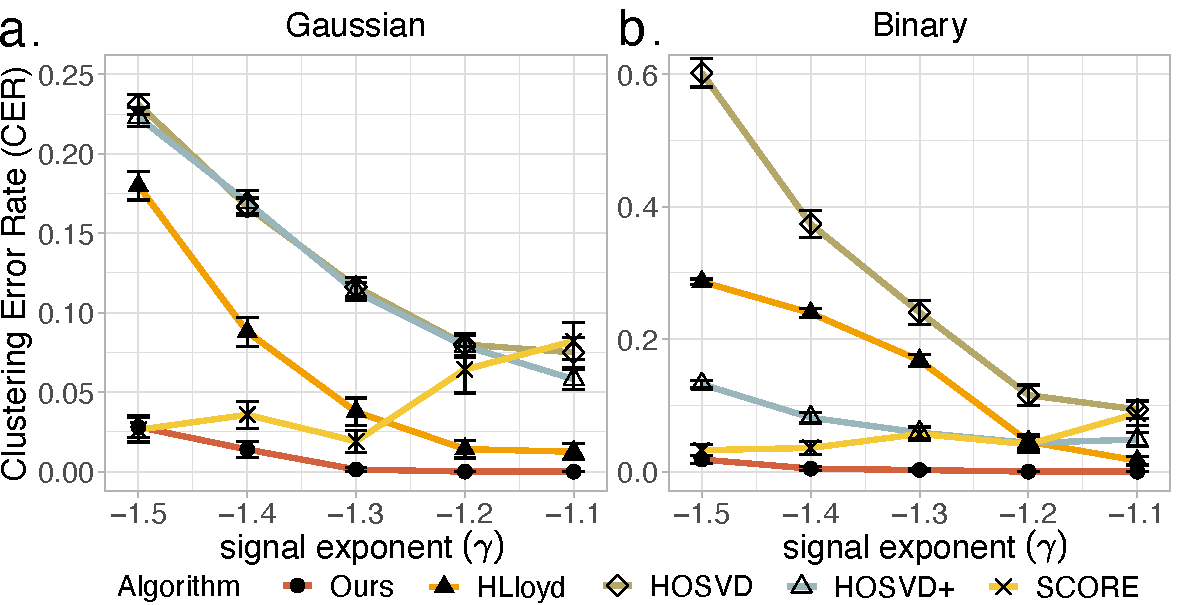
\includegraphics[width=.48\textwidth]{comp_gamma_anno2.pdf}
%DIFDELCMD <     %%%
%DIFDELCMD < \caption{%
{%DIFAUXCMD
%DIFDELCMD < \footnotesize %%%
\DIFdelFL{CER versus signal exponent (denoted $\gamma$) for different methods. We set $p = 100, r = 5, \gamma \in [-1.5, -1.1]$ under (a) Gaussian and (b) Bernoulli models.}}
    %DIFAUXCMD
%DIFDELCMD < \label{fig:comp_gamma}
%DIFDELCMD < \end{figure}
%DIFDELCMD < 

%DIFDELCMD < \begin{figure}
%DIFDELCMD <     \centering
%DIFDELCMD <     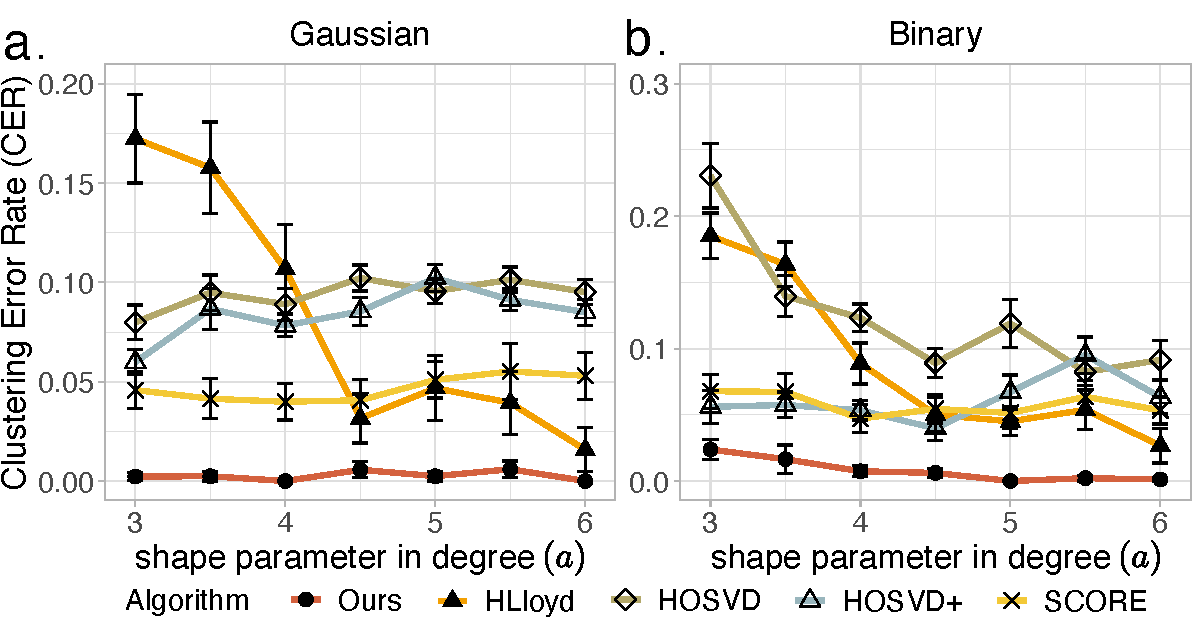
\includegraphics[width=.48\textwidth]{comp_theta_anno2.pdf}
%DIFDELCMD <     %%%
%DIFDELCMD < \caption{%
{%DIFAUXCMD
%DIFDELCMD < \footnotesize %%%
\DIFdelFL{CER versus shape parameter in degree (denoted $a\in[3,6]$) for different methods. We set $p = 100, r = 5, c= 0.5, \gamma = -1.2$ under (a) Gaussian and (b) Bernoulli models.}}
    %DIFAUXCMD
%DIFDELCMD < \label{fig:comp_theta}
%DIFDELCMD <         \vspace{-.4cm}
%DIFDELCMD < \end{figure}
%DIFDELCMD < 

%DIFDELCMD < %%%
\DIFdelend The last experiment investigates the effects of degree heterogeneity to clustering performance. We \DIFaddbegin \DIFadd{use the same setting as in the first experiment in the Section~\ref{subsec:comp}, except that we }\DIFaddend fix the signal exponent $\gamma = -1.2$ and \DIFdelbegin \DIFdel{vary the extent of degree heterogeneity . In this experiment, we generate }\DIFdelend \DIFaddbegin \DIFadd{generate the degree heterogeneity }\DIFaddend $\mtheta$ from Pareto distribution prior to normalization. The density function of Pareto distribution is $f(x|a,b) = a b^a x^{-(a+1)} \ind\{ x \geq b \}$, where $a$ is called \emph{shape} parameter. We vary \DIFaddbegin \DIFadd{the shape parameter }\DIFaddend $a \in [3,6]$ and choose $b$ such that \DIFdelbegin \DIFdel{$\bbE[X] = a(a - 1)^{-1}b = 1$ }\DIFdelend \DIFaddbegin \DIFadd{$\bbE X = a(a - 1)^{-1}b = 1$ }\DIFaddend for $X$ following Pareto$(a,b)$. Note that a smaller $a$ leads to a larger variance in $\mtheta$ and hence a larger degree heterogeneity. \DIFdelbegin \DIFdel{Fig.}\DIFdelend \DIFaddbegin \DIFadd{Figure}\DIFaddend ~\ref{fig:comp_theta} demonstrates the stability of degree-corrected algorithms (\textbf{\small dTBM}, \textbf{\small SCORE}, \textbf{\small HOSVD+}) over the entire range of degree heterogeneity under consideration. In contrast, non-degree algorithms (\textbf{\small HLloyd}, \textbf{\small HOSVD}) show poor performance with large heterogeneity, especially in Bernoulli cases. This experiment, again, highlights the benefit of addressing degree heterogeneity in \DIFdelbegin \DIFdel{higher-order }\DIFdelend clustering. 

%DIF < We fix the signal with $\alpha = 2$ and set $c = 1$ and $c = 0.25$ for Gaussian and Bernoulli cases, respectively.   Fig.~\ref{fig:comp_theta} demonstrates the outstanding performance of \textbf{\small dTBM} and \textbf{\small SCORE} under all range of degree heterogeneity. Specifically, \textbf{\small SCORE} slightly beats \textbf{\small dTBM} in Gaussian case. A possible reason for the outperformance is that \textbf{\small SCORE} purposes a relaxer constrain on $\mtheta$. The terrible performances of \textbf{\small HLloyd} and \textbf{\small HOSVD+} confirm the failure of non-degree algorithms  facing strong heterogeneity.
\DIFaddbegin \begin{figure}[htb]
 \vspace{-.3cm}
    \centering
    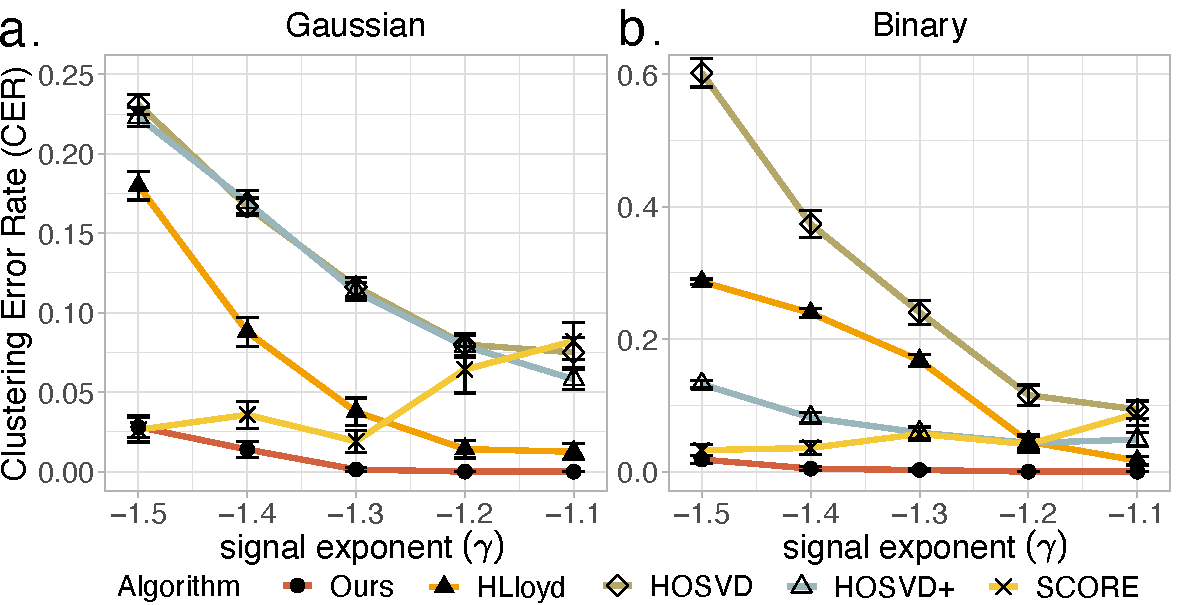
\includegraphics[width=.95\columnwidth]{comp_gamma_anno2.pdf}
    \caption{ \footnotesize \DIFaddFL{CER versus signal exponent (denoted $\gamma$) for different methods. We set $p = 100, r = 5, \gamma \in [-1.5, -1.1]$ under (a) Gaussian and (b) Bernoulli models.}}
    \label{fig:comp_gamma}
    \vspace{-.4cm}
\end{figure}
\DIFaddend 

\DIFdelbegin \subsection{\DIFdel{Peru Legislation data analysis}}
%DIFAUXCMD
\addtocounter{subsection}{-1}%DIFAUXCMD
\DIFdelend \DIFaddbegin \begin{figure}[htb]
\vspace{-.2cm}
    \centering
    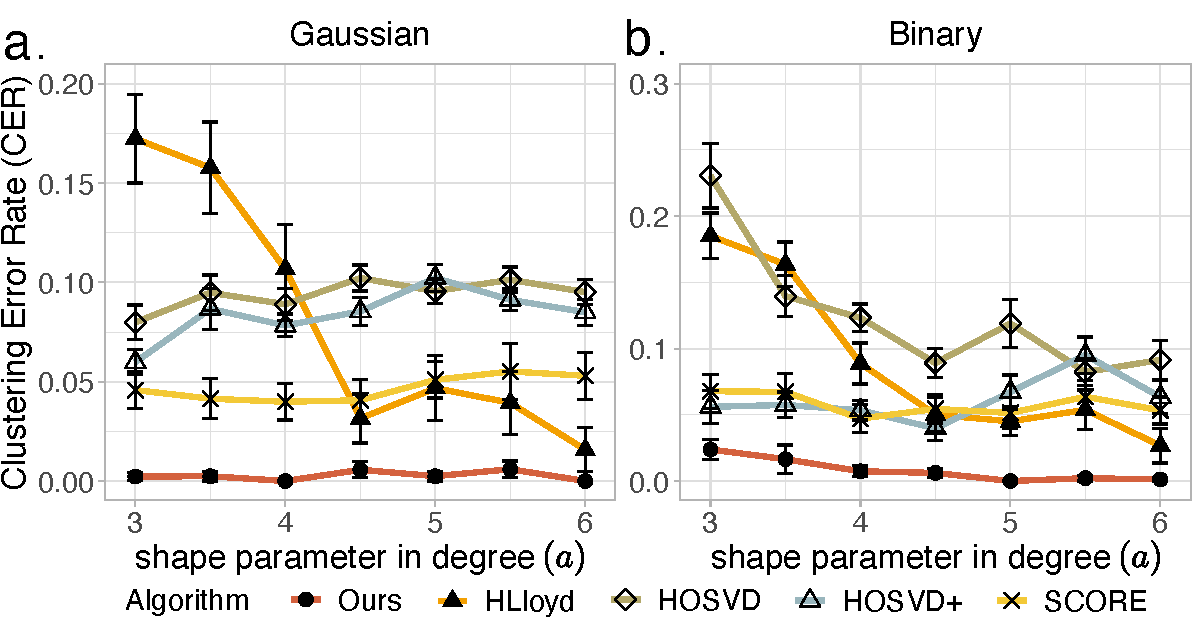
\includegraphics[width=.95\columnwidth]{comp_theta_anno2.pdf}
    \caption{ \footnotesize \DIFaddFL{CER versus shape parameter in degree (denoted $a\in[3,6]$) for different methods with $p = 100, r = 5, \gamma = -1.2$ under (a) Gaussian and (b) Bernoulli models.}}
    \label{fig:comp_theta}
    \vspace{-.3cm}
\end{figure}
\DIFaddend 

\DIFdelbegin \DIFdel{We consider }\DIFdelend %DIF > \section{REAL DATA}\label{sec:real}
\DIFaddbegin 

\subsection{\DIFadd{Peru Legislation Data Analysis}}

\DIFadd{We apply our method to }\DIFaddend the legislation networks in the Congress of the Republic of Peru \citep{lee2017time}. Because of the frequent political power shifts in the Peruvian Congress during 2006-2011, we choose to focus on the data for the first half of 2006-2007 year. The dataset records the co-sponsorship of 116 legislators from top 5 parties and 802 bill proposals. We reconstruct legislation network as an order-3 binary tensor $\tY \in \{0,1\}^{116 \times 116 \times 116}$, where $\tY_{ijk} = 1$ if the legislators $(i,j,k)$ have sponsored the same bill, and $\tY_{ijk} = 0$ otherwise. \DIFdelbegin \DIFdel{The true }\DIFdelend \DIFaddbegin \DIFadd{True }\DIFaddend party affiliations of legislators are provided and serve as \DIFaddbegin \DIFadd{the }\DIFaddend ground truth. We apply various higher-order clustering methods to $\tY$ with $r = 5$. \DIFdelbegin \DIFdel{Tab.}\DIFdelend \DIFaddbegin \DIFadd{Table}\DIFaddend ~\ref{tab:peru} shows that our \textbf{\small dTBM} achieves the best performance compared to others. The second best method is the two-stage algorithm \textbf{\small HLloyd}, followed by the spectral methods \textbf{\small SCORE} and \textbf{\small HOSVD+}\DIFdelbegin \DIFdel{. This result is consistent with our }\DIFdelend \DIFaddbegin \DIFadd{, which consists with }\DIFaddend simulations under strong signal and moderate degree heterogeneity. 
\DIFdelbegin \DIFdel{The comparison suggests that our method }\textbf{%DIFDELCMD < \small %%%
\DIFdel{dTBM}} %DIFAUXCMD
\DIFdel{is more appealing in real-world applications.
}%DIFDELCMD < 

%DIFDELCMD < %%%
%DIF < We consider the legislation networks in the Congress of the Republic of Peru \citep{lee2017time}. The data records the co-sponsorship of 130 legislators for 28422 bill proposals from 2006 to 2010 and the true party affiliations of the legislators. Note that power shifts in the Peruvian Congress occurred frequently during this period. Thus, we focus on the bills proposed in first half of 2006-2007 political year and legislators from the top 5 parties with at least 5 members in the Congress. The network eventually includes 116 legislator and 802 bill proposals. We reconstruct an order-3 binary tensor $\tY \in \{0,1\}^{116 \times 116 \times 116}$ from the original network data, where the entries indicate the existence of co-sponsorship among legislators. Specifically, we let $\tY_{ijk} = 1$ if the legislators $i,j,k$ have sponsored the same bill, otherwise, we let $\tY_{ijk} = 0$. To reveal the party affiliation of legislators, we apply multiple tensor clustering methods to $\tY$ with the number of communities $r = 5$.
%DIFDELCMD < 

%DIFDELCMD < %%%
%DIF < Table~\ref{tab:peru} collects the clustering performance of each method, where the true party affiliation serves as the true assignment to calculate CER. We can see our algorithm substantially outperforms than other methods with the lowest CER of 0.116. The \textbf{HLloyd} method is the second best with CER 0.149, where the underperformance indicates the necessity to introduce degree corrected parameters. The other spectral clustering methods only achieve CER around 0.2. This indicates that Lloyd-based methods may be more appealing in practice.
%DIFDELCMD < 

%DIFDELCMD < \begin{table}[hbt]
%DIFDELCMD <     %%%
\DIFdelendFL %DIF > The comparison suggests that our method \textbf{\small dTBM} is more appealing in real-world applications.
\DIFaddbeginFL \vspace{-.5cm}
\begin{table}[ht]
    \DIFaddendFL \centering
    \DIFdelbeginFL %DIFDELCMD < \begin{tabular}{c |c c c c}
%DIFDELCMD <     \hline
%DIFDELCMD <         %%%
\DIFdelFL{Method }%DIFDELCMD < & %%%
\textbf{%DIFDELCMD < \small %%%
\DIFdelFL{dTBM}} %DIFAUXCMD
%DIFDELCMD < &   %%%
\textbf{%DIFDELCMD < \small %%%
\DIFdelFL{HOSVD+}} %DIFAUXCMD
%DIFDELCMD < & %%%
\textbf{%DIFDELCMD < \small %%%
\DIFdelFL{HLloyd}} %DIFAUXCMD
%DIFDELCMD < &  %%%
\textbf{%DIFDELCMD < \small %%%
\DIFdelFL{SCORE}}%DIFAUXCMD
%DIFDELCMD < \\
%DIFDELCMD <          %%%
\DIFdelFL{CER }%DIFDELCMD < & %%%
\textbf{\DIFdelFL{0.116}} %DIFAUXCMD
%DIFDELCMD < &%%%
\DIFdelFL{0.213 }%DIFDELCMD < & %%%
\DIFdelFL{0.149 }%DIFDELCMD < &%%%
\DIFdelFL{0.199}%DIFDELCMD < \\
%DIFDELCMD <          \hline
%DIFDELCMD <     \end{tabular}
%DIFDELCMD <     %%%
\DIFdelendFL \DIFaddbeginFL \resizebox{\columnwidth}{!}{%
    \begin{tabular}{c | c cc c}
    \hline
        Method & \textbf{\small dTBM} 
     %   &\textbf{\small HOSVD}
        &\textbf{\small HOSVD+} & \textbf{\small HLloyd} &  \textbf{\small SCORE}\\
         CER & \textbf{0.116}
   %      &  0.22 
         &0.213 & 0.149 &0.199\\
         \hline
    \end{tabular}
    }
    \vspace{-.3cm}
    \DIFaddendFL \caption{ \footnotesize Clustering errors (measured by CER) for various methods in the analysis of Peru Legislation dataset.}
    \label{tab:peru}
\end{table}




%DIF <  \begin{table}[hbt]
%DIF <      \centering
%DIF <      \begin{tabular}{c |c c c}
%DIF <      \hline
%DIF <          Method & \textbf{\small Ours} &   \textbf{\small HOSVD} & \textbf{\small HOSVD+}\\
%DIF <           CER & \textbf{0.116} & 0.22 &0.213 \\
%DIF <           \hline
%DIF <           Method & \textbf{\small HLloyd} &\textbf{\small SCORE} & \textbf{\small SCORE-} \\
%DIF <           CER &0.149 &  0.199 & 0.228\\
%DIF <           \hline
%DIF <      \end{tabular}
%DIF <      \caption{CER of real data for different methods.}
%DIF <      \label{tab:peru}
%DIF <  \end{table}
\DIFaddbegin \thispagestyle{empty}
\DIFaddend 

\DIFdelbegin %DIFDELCMD < \vspace{-0.5cm}
%DIFDELCMD < %%%
\section{\DIFdel{Conclusion}}
%DIFAUXCMD
\addtocounter{section}{-1}%DIFAUXCMD
\DIFdel{We have developed a general degree-corrected tensor block model with a two-step angle-based polynomial-times algorithm. We have, for the first time, characterized the statistical and computational behaviors of the degree-corrected tensor block model under different signal-to-noise ratio regimes. Simulations and Peru Legislation data analysis confirm the potential of our method for practical applications. 
%DIF < The gap of statistical and computational limits reveals the inherent distinctions between higher-order clustering and matrix clustering. We also have provided , which is guaranteed to achieve exact clustering under mild signal conditions. 
}\DIFdelend \DIFaddbegin \subsection*{\DIFadd{Acknowledgments}}
\DIFadd{This research is supported in part by NSF grants DMS-1915978, DMS-2023239, EF-2133740, and funding from the Wisconsin Alumni Research foundation. We thank Zheng Tracy Ke, Rungang Han, Yuetian Luo for helpful discussions and for sharing software packages. 
}

\thispagestyle{empty}
\DIFaddend 

\bibliographystyle{apalike}
\bibliography{tensor_wang}

\end{document}
